\section{サブシステムの概要}

本システムは、以下のサブシステムにより構成する。
各サブシステムは共通のデータベースを参照・更新し、登録された情報を利用者の権限に応じて提供する。

\begin{itemize}
    \item 大会情報管理サブシステム：大会の作成、編集、公開および開催状況の管理を行う。
    \item 競技者登録・管理サブシステム：競技者アカウント、参加登録、競技者一覧および受付状況を管理する。
    \item トーナメント・試合管理サブシステム：対戦組み合わせの作成、試合結果の登録・確認、大会進行状況の更新を行う。
    \item 観戦者向け情報提供サブシステム：大会全体や選手ごとの試合状況、成績、対戦履歴およびYouTube、Xなどの配信情報を提供する。
    \item 通知サブシステム：試合予定の変更や試合結果の更新などをメールで通知する。
\end{itemize}

\subsection{大会情報管理サブシステム}
主催者が大会情報を登録・管理し、競技者および観戦者に公開する。

\subsubsection*{(a) 大会作成・編集機能}
\begin{description}
    \item[入力：]大会名、対象ゲーム、開催日時、開催場所、最大参加人数、大会形式、参加受付期間、参加条件、ルール等、大会全体の配信URL
    \item[出力：]大会情報、公開情報
    \item[処理：]主催者が入力した大会情報を確認し、データベースに保存する。
                大会形式はシングルエリミネーションまたは総当たり方式とする。
                大会全体の配信を行う場合は、配信URLを登録し、
                大会詳細画面および大会観戦画面に表示する。
\end{description}

\begin{figure}[H]
    \centering
    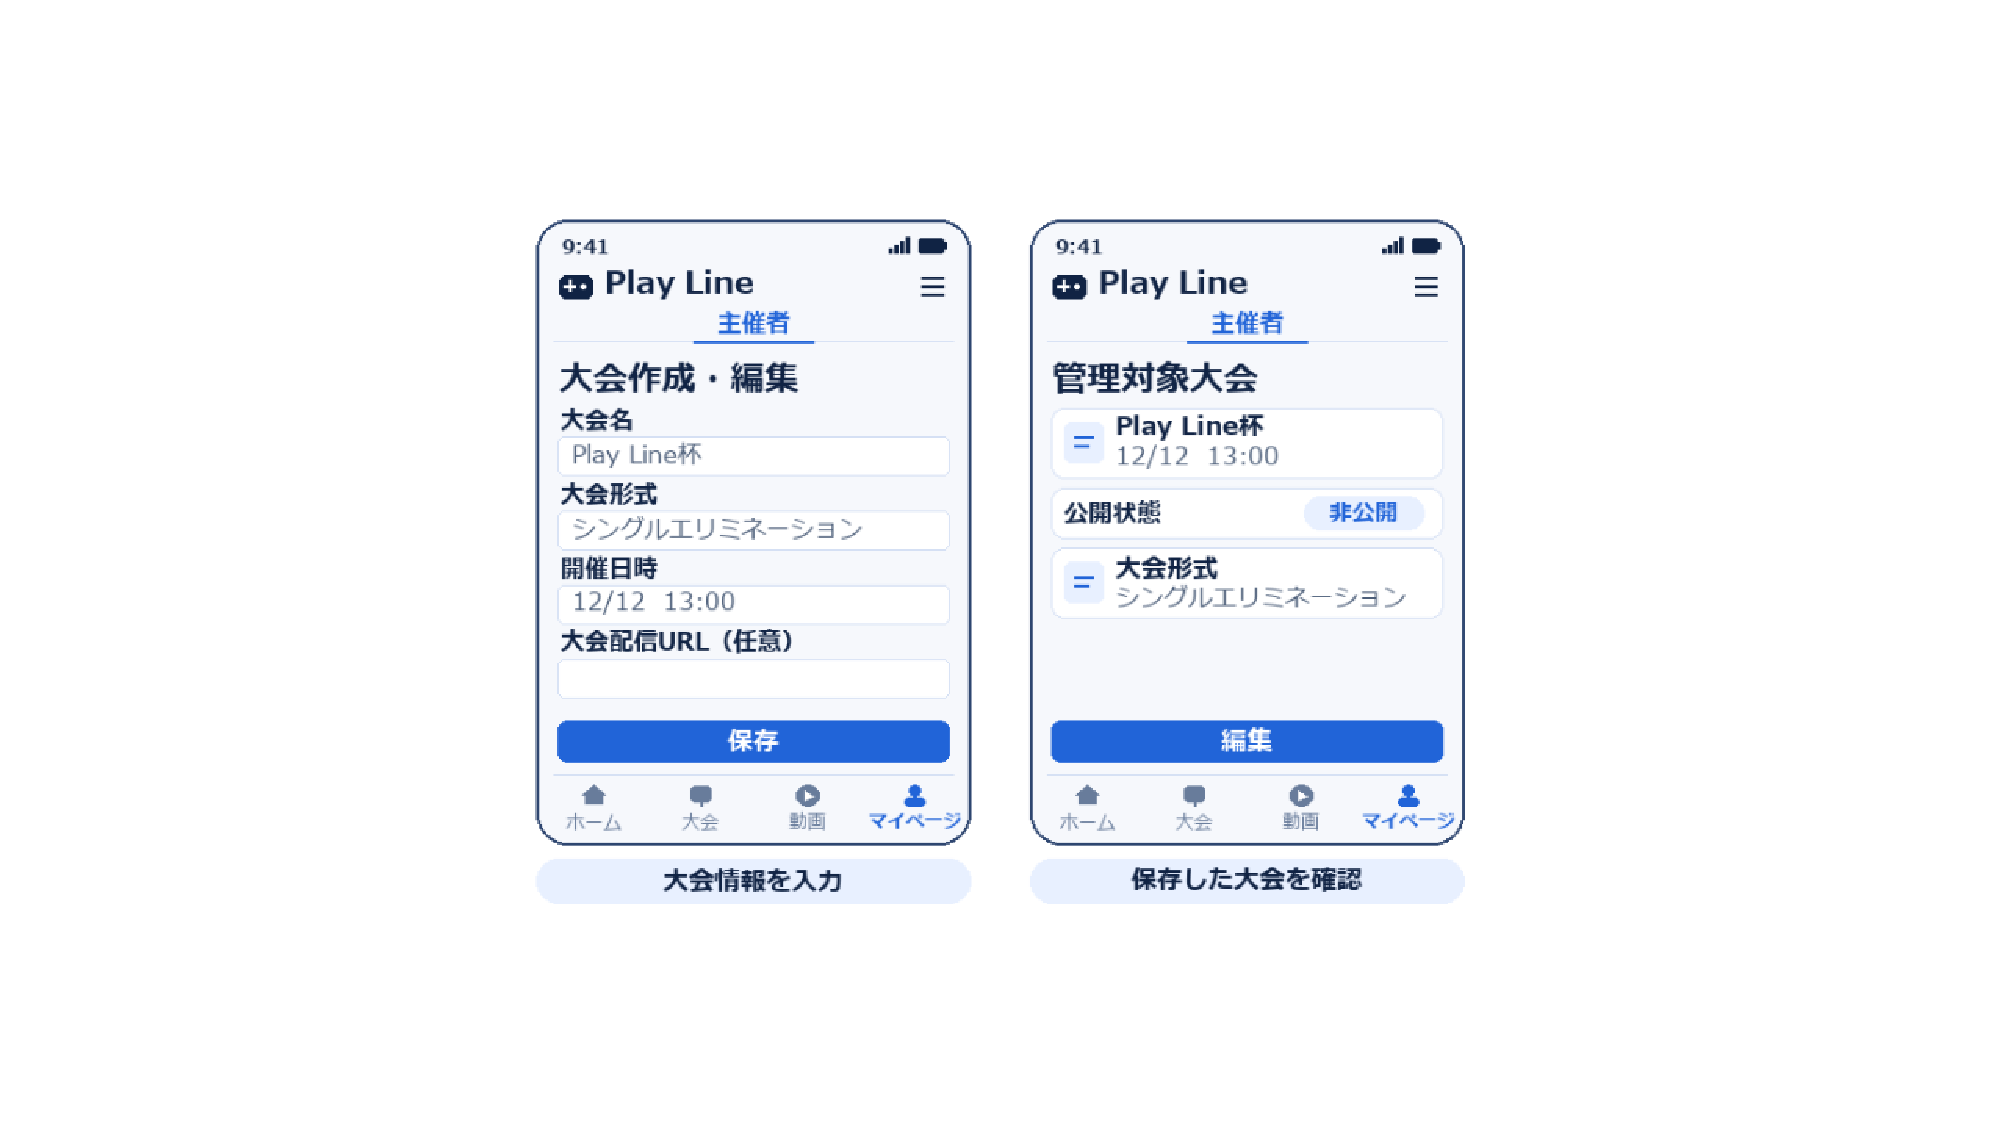
\includegraphics[width=\linewidth]{figures/03/3-1_edit.pdf}
    \caption{大会作成・編集画面イメージ}
    \label{fig:tournament_edit_ui}
\end{figure}

\subsubsection*{(b) 大会検索・一覧表示機能}
\begin{description}
    \item[入力：]大会名、対象ゲーム、開催日、開催状況等の検索条件
    \item[出力：]条件に一致する大会一覧
    \item[処理：]公開されている大会情報を検索し、開催予定・開催中・終了済みなどの状態とともに表示する。
\end{description}

\begin{figure}[H]
    \centering
    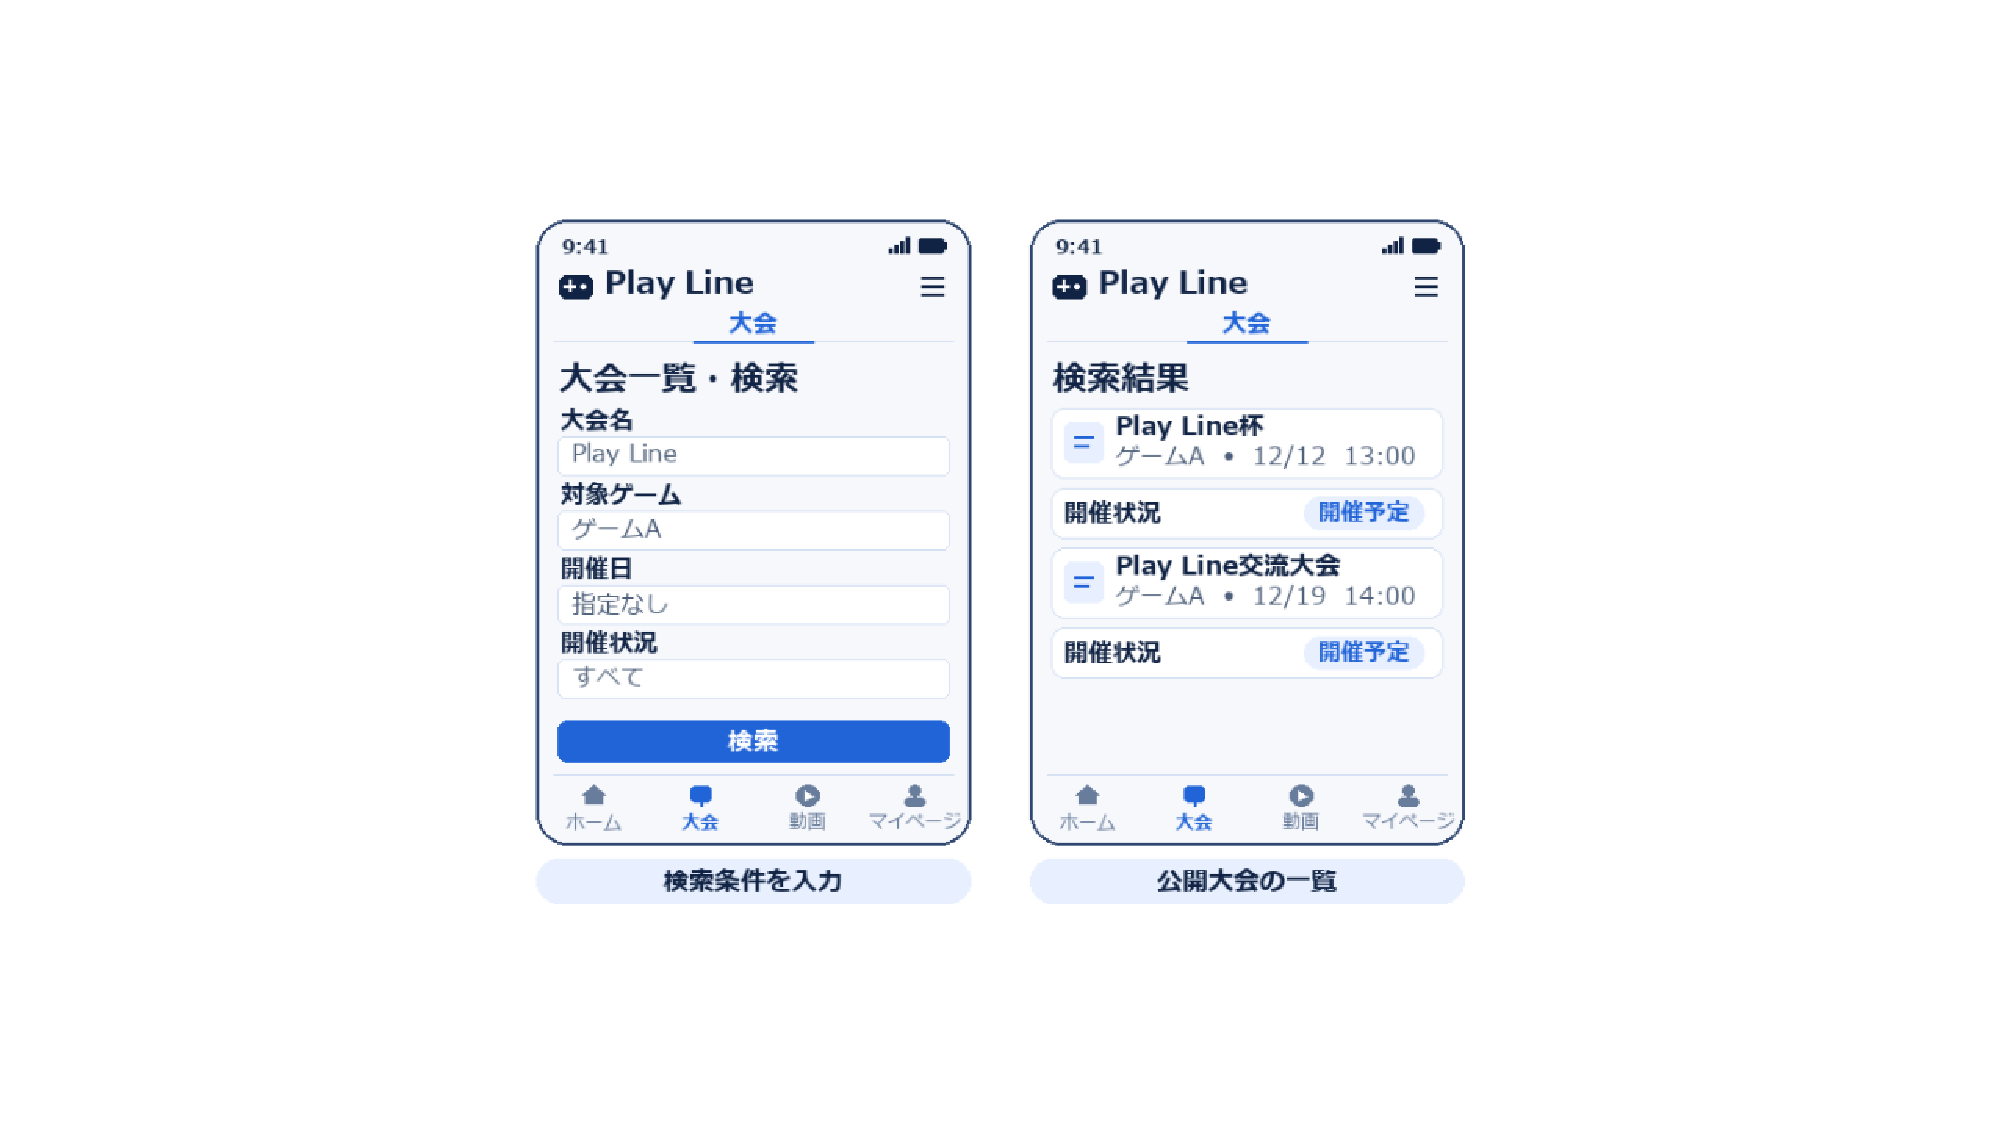
\includegraphics[width=\linewidth]{figures/03/3-1_search.pdf}
    \caption{大会検索・一覧画面イメージ}
    \label{fig:tournament_search_ui}
\end{figure}

\subsubsection*{(c) 大会進行情報表示機能}
\begin{description}
    \item[入力：]大会ID
    \item[出力：]大会の進行状況、試合一覧、トーナメント表
    \item[処理：]大会に関連付けられた試合情報と結果を参照し、現在の進行状況を表示する。
\end{description}

\begin{figure}[H]
    \centering
    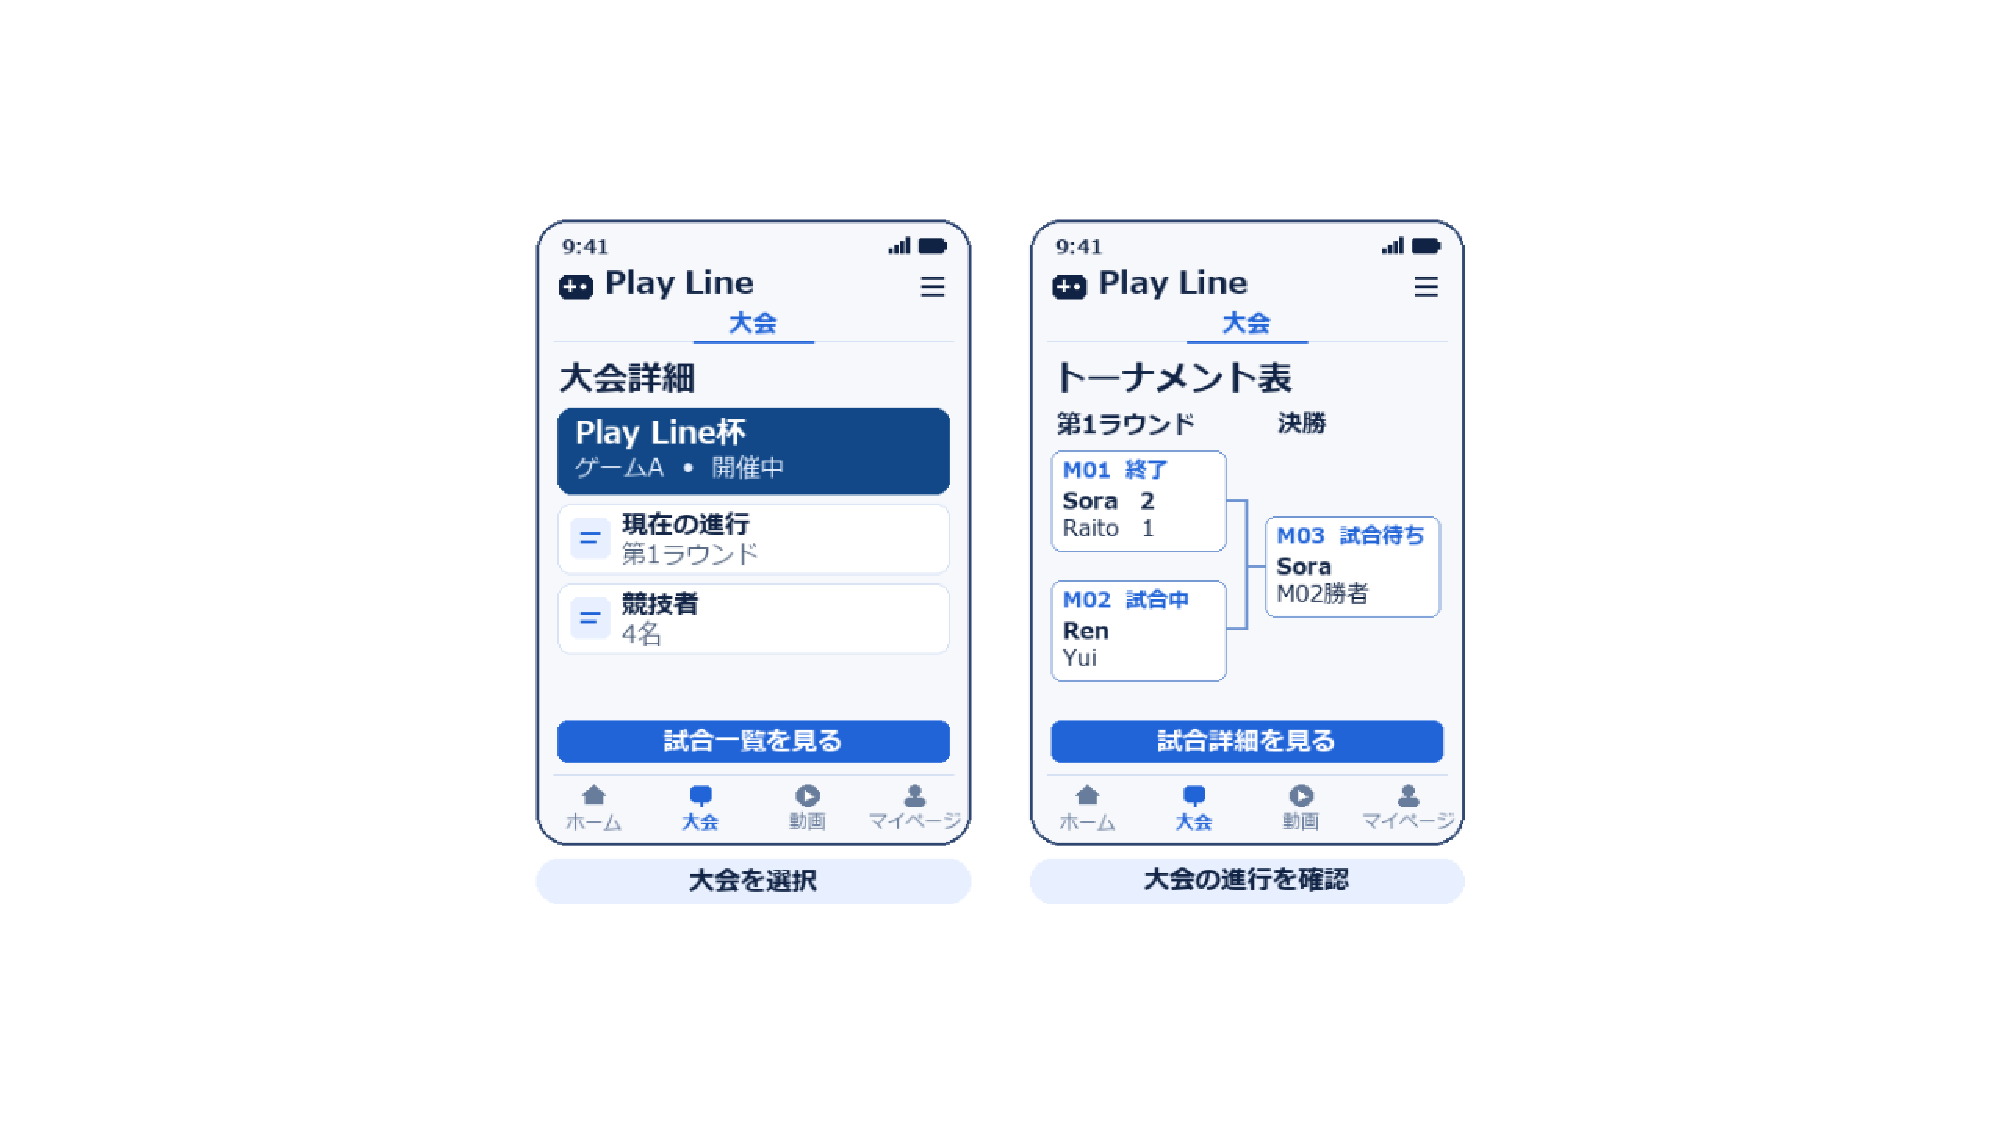
\includegraphics[width=\linewidth]{figures/03/3-1_detail.pdf}
    \caption{大会進行情報画面イメージ}
    \label{fig:tournament_detail_ui}
\end{figure}

\subsection{競技者登録・管理サブシステム}
競技者のアカウント情報および大会への参加情報を管理する。

\subsubsection*{(a) 競技者アカウント登録機能}
\begin{description}
    \item[入力：]氏名、プレイヤー名、メールアドレス、ログイン情報等
    \item[出力：]登録結果、競技者ID
    \item[処理：]入力内容の必須項目、形式および既存情報との重複を確認し、
                問題がなければ競技者情報を保存する。
\end{description}

\begin{figure}[H]
    \centering
    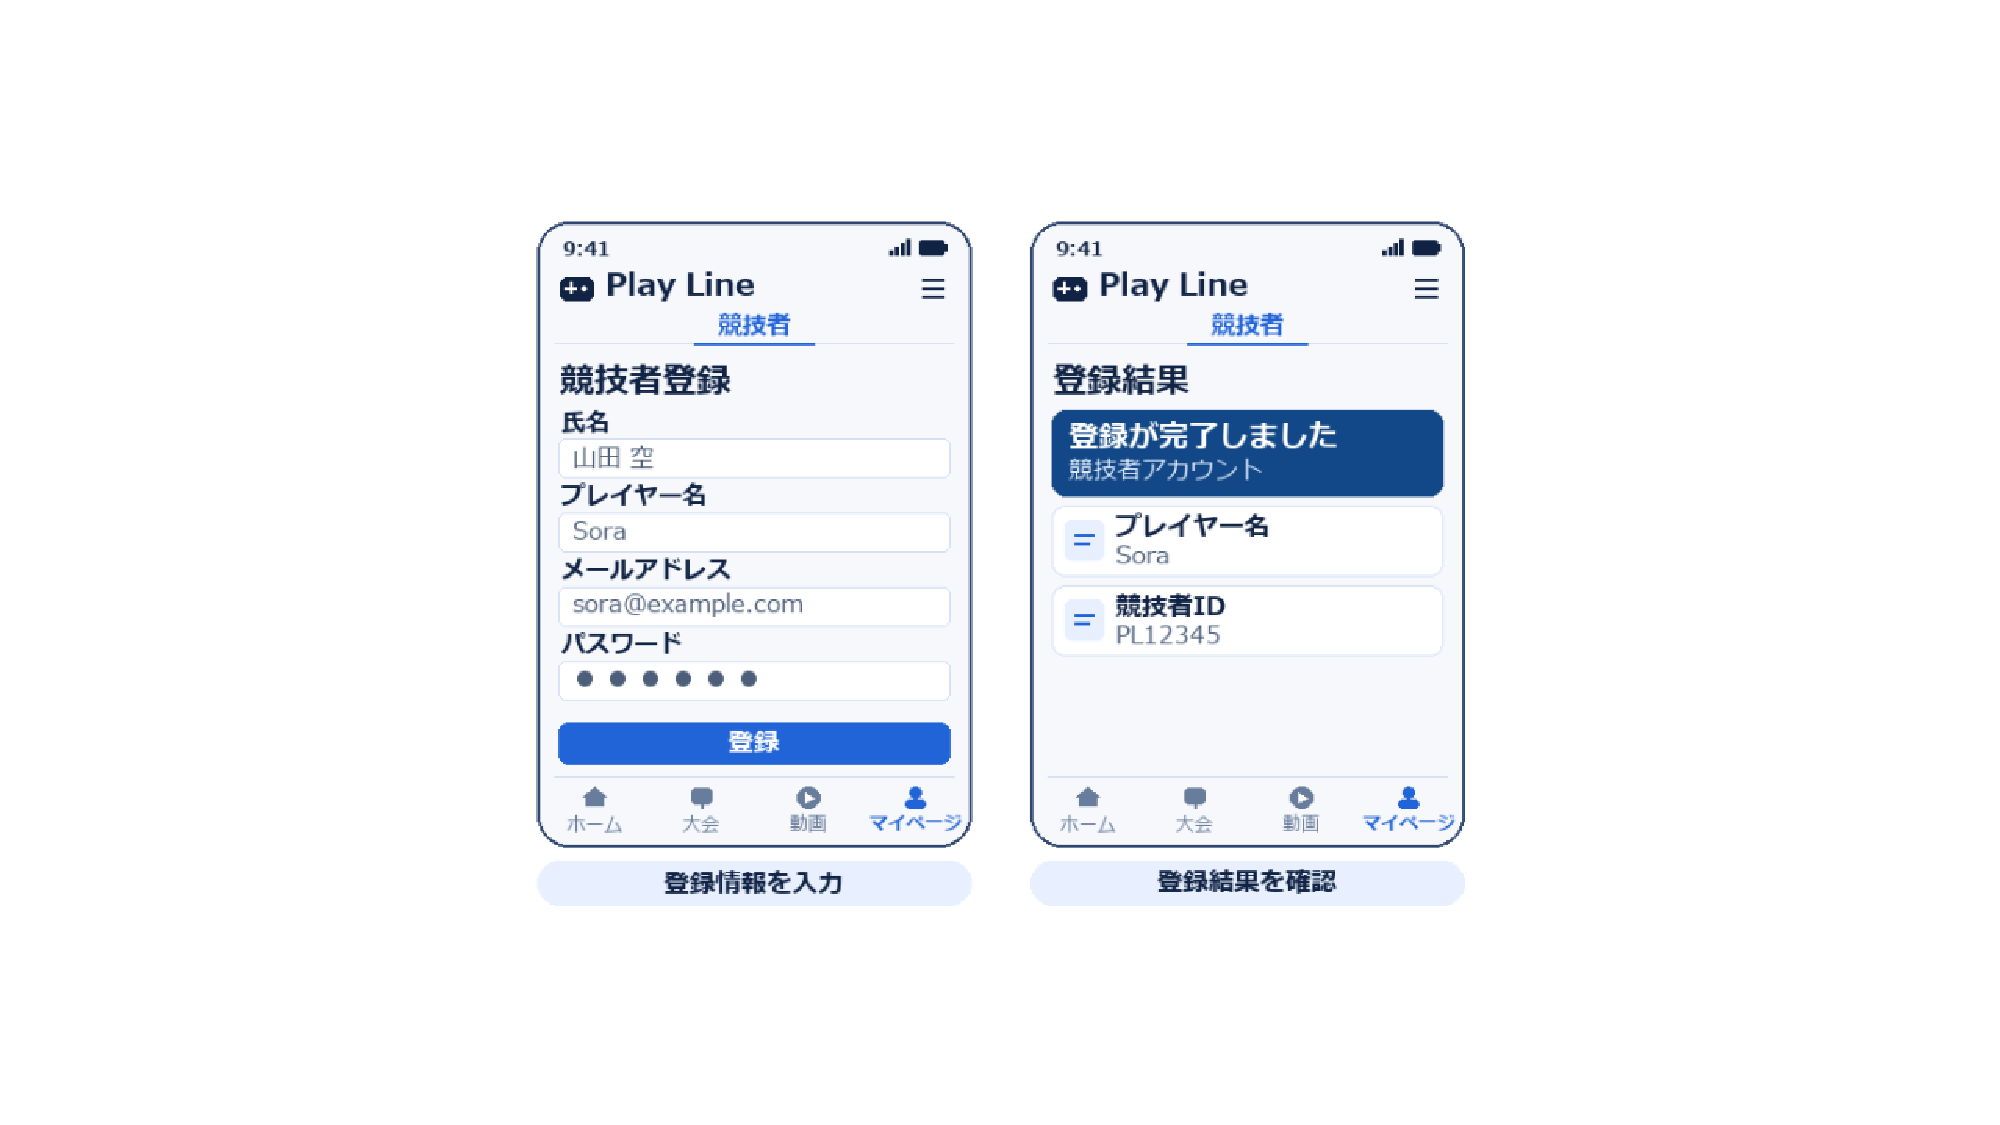
\includegraphics[width=\linewidth]{figures/03/3-2_register.pdf}
    \caption{競技者アカウント登録画面イメージ}
    \label{fig:player_register_ui}
\end{figure}

\subsubsection*{(b) 大会参加登録機能}
\begin{description}
    \item[入力：]大会ID、競技者ID、参加登録に必要な情報
    \item[出力：]参加登録結果
    \item[処理：]参加受付期間や定員などの大会条件を確認し、参加情報をデータベースに登録する。
\end{description}

\begin{figure}[H]
    \centering
    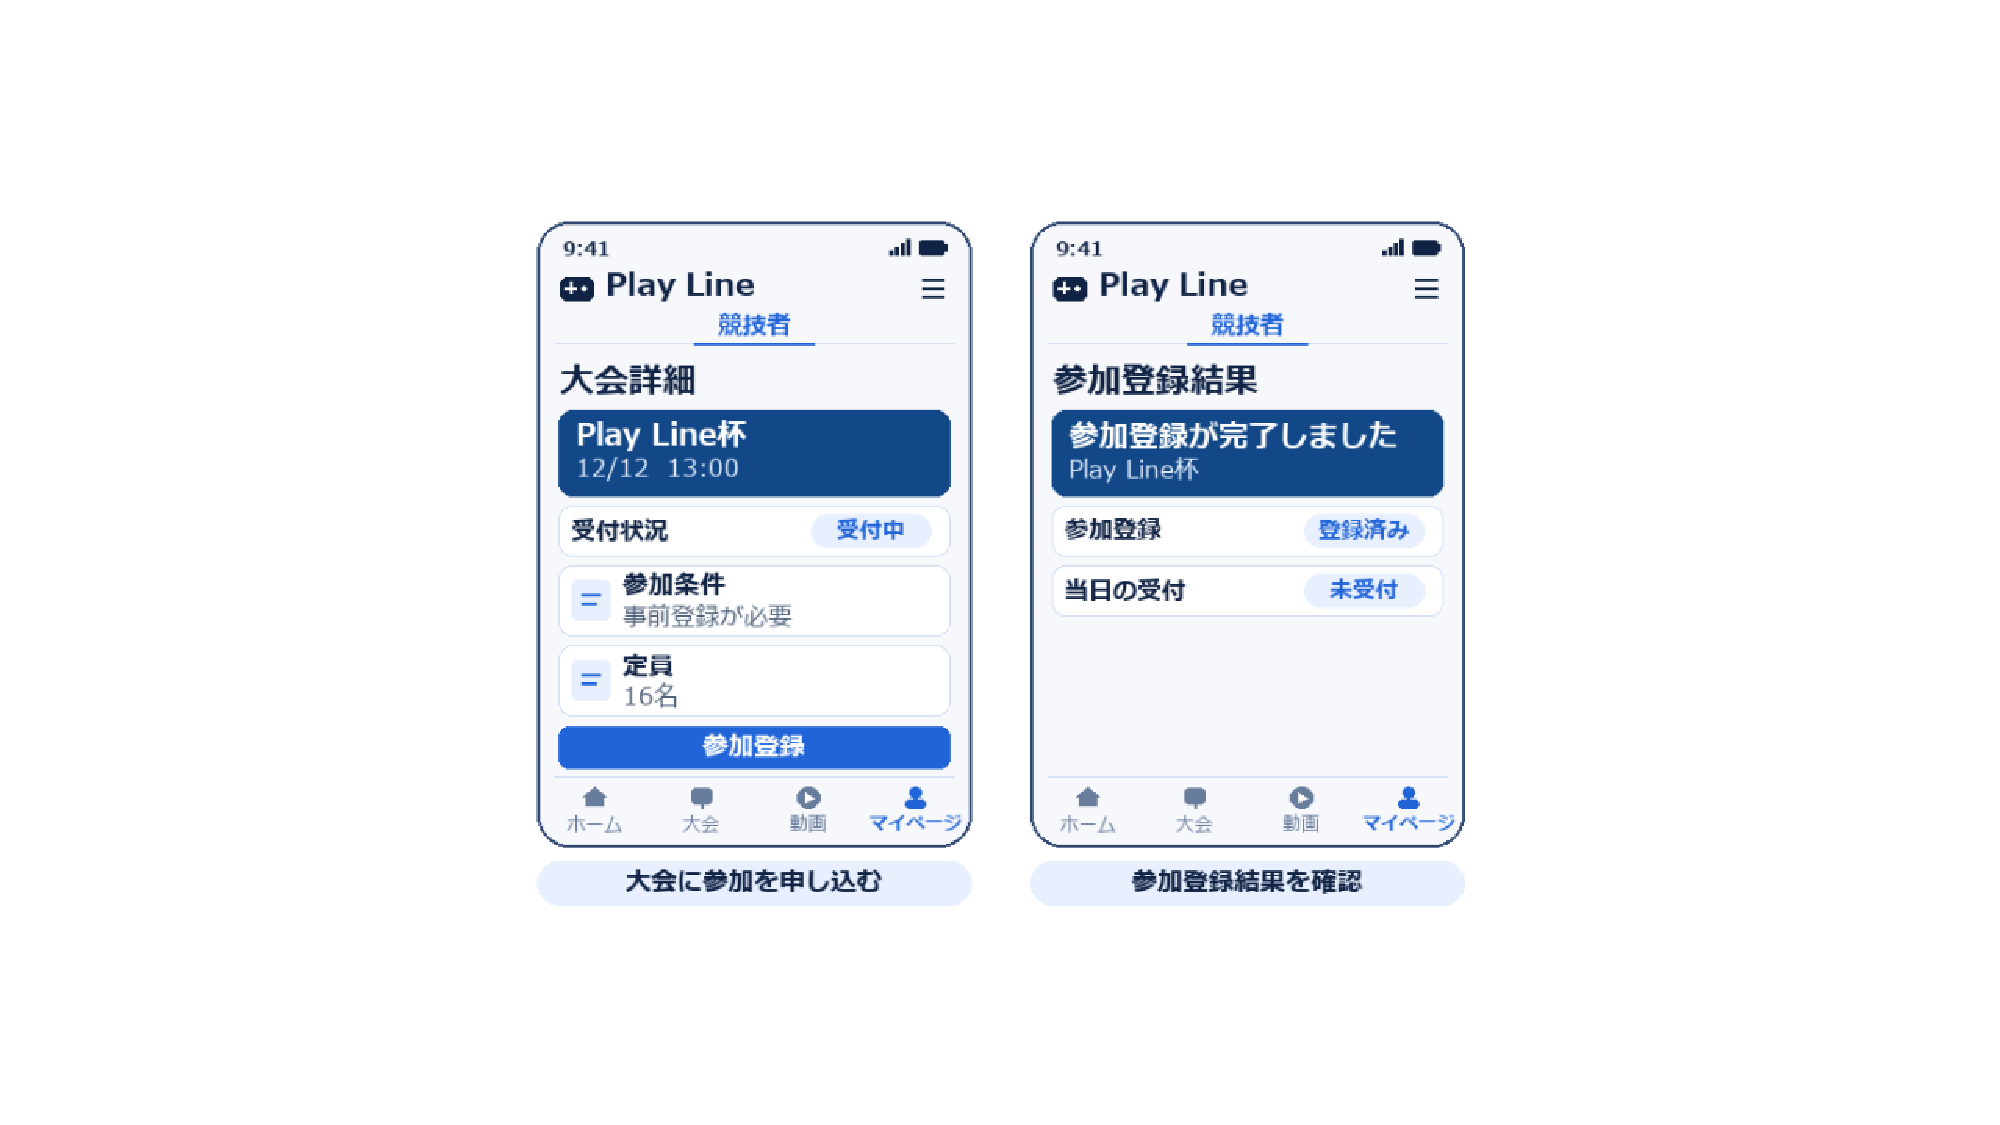
\includegraphics[width=\linewidth]{figures/03/3-2_entry.pdf}
    \caption{大会参加登録画面イメージ}
    \label{fig:tournament_entry_ui}
\end{figure}

\subsubsection*{(c) 競技者管理・受付機能}
\begin{description}
    \item[入力：]大会ID、競技者ID、受付状態
    \item[出力：]競技者一覧、受付済み/未受付の状態
    \item[処理：]主催者に競技者一覧を表示する。
                主催者が確認した競技者について受付状態を更新する。
                参加登録と受付完了は別の状態として管理する。
\end{description}

\begin{figure}[H]
    \centering
    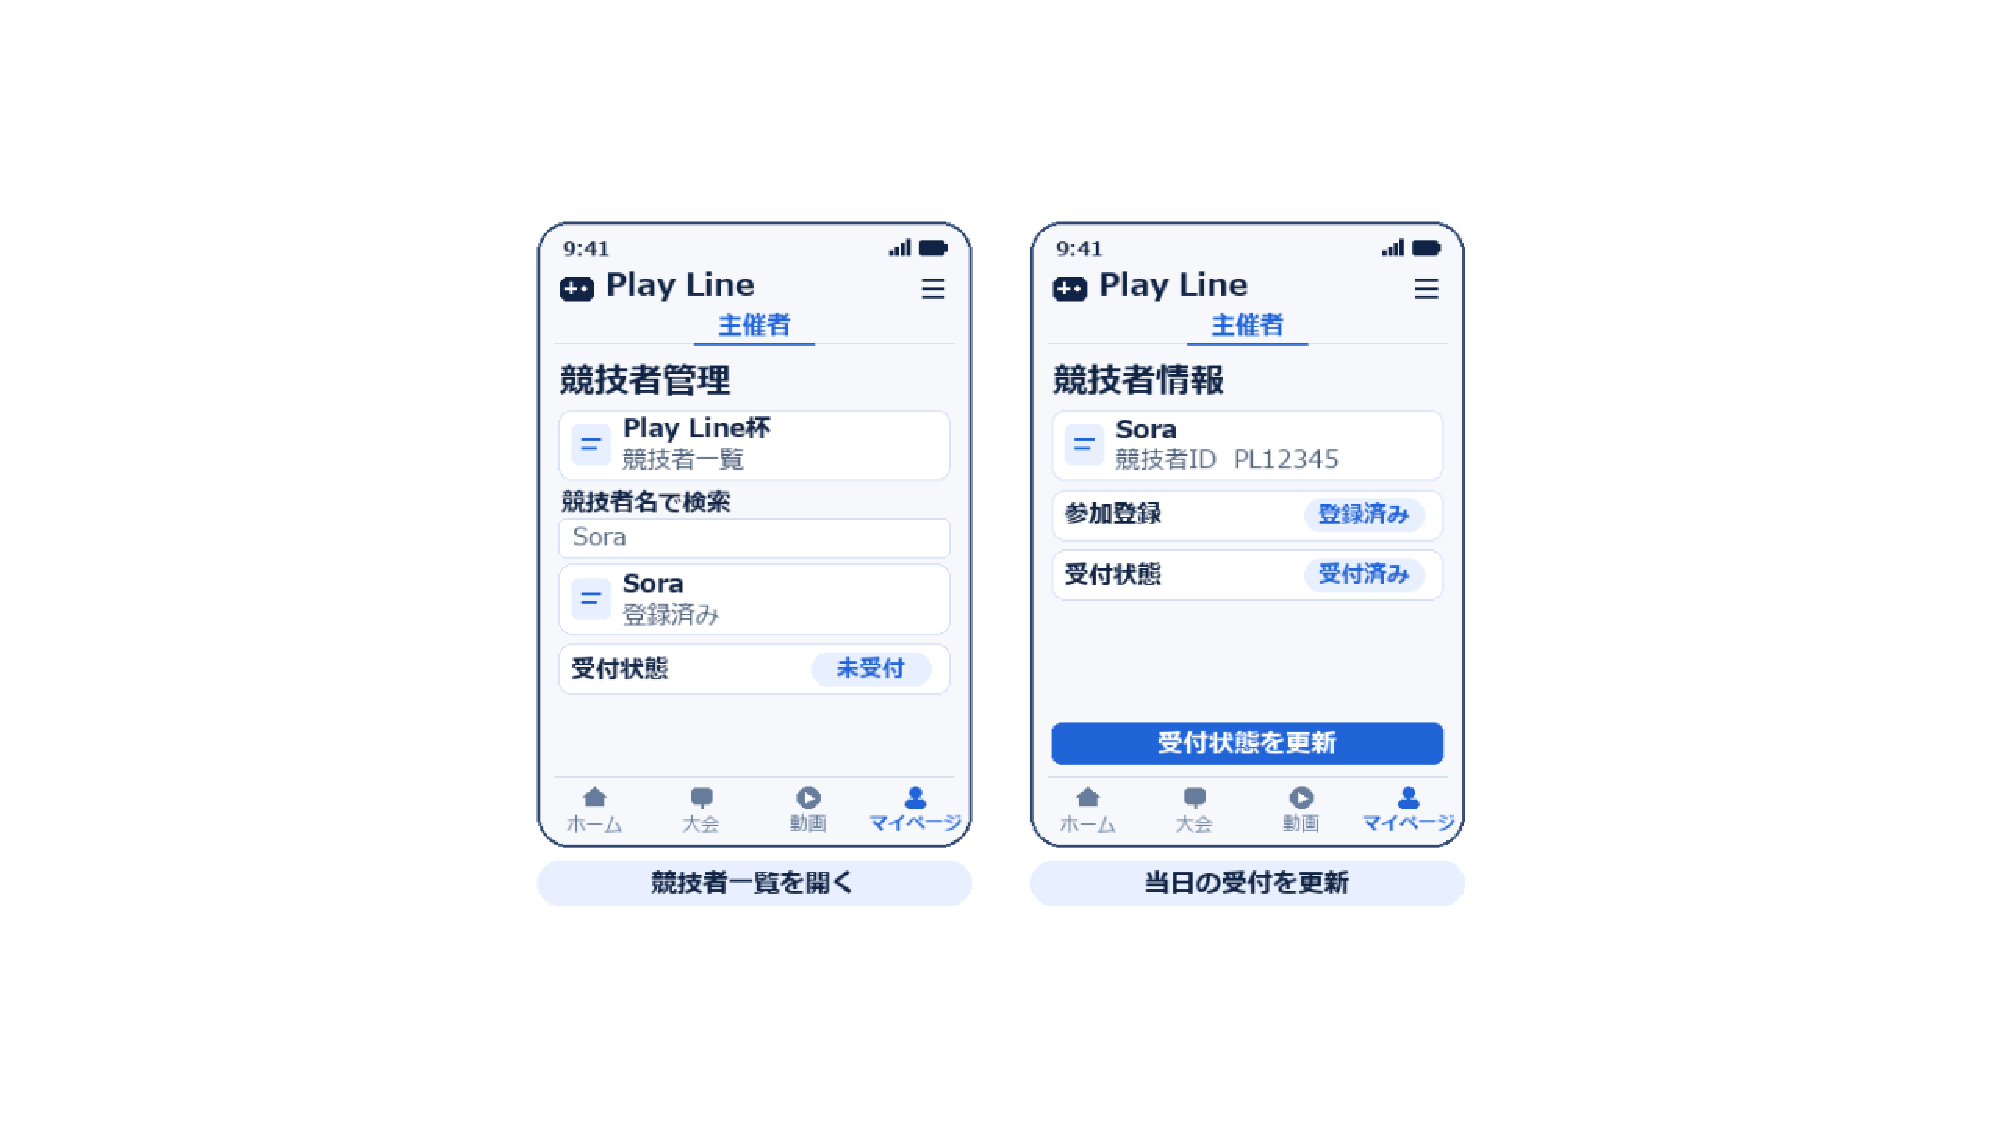
\includegraphics[width=\linewidth]{figures/03/3-2_manage.pdf}
    \caption{競技者管理・受付画面イメージ}
    \label{fig:player_manage_ui}
\end{figure}

\subsubsection*{(d) 競技者向け試合情報確認機能}
\begin{description}
    \item[入力：]ログイン中の競技者ID、大会ID
    \item[出力：]本人の対戦相手、試合予定、試合結果、トーナメント上の位置
    \item[処理：]本人が参加する大会および試合情報を検索し、競技者向け画面に表示する。
\end{description}

\begin{figure}[H]
    \centering
    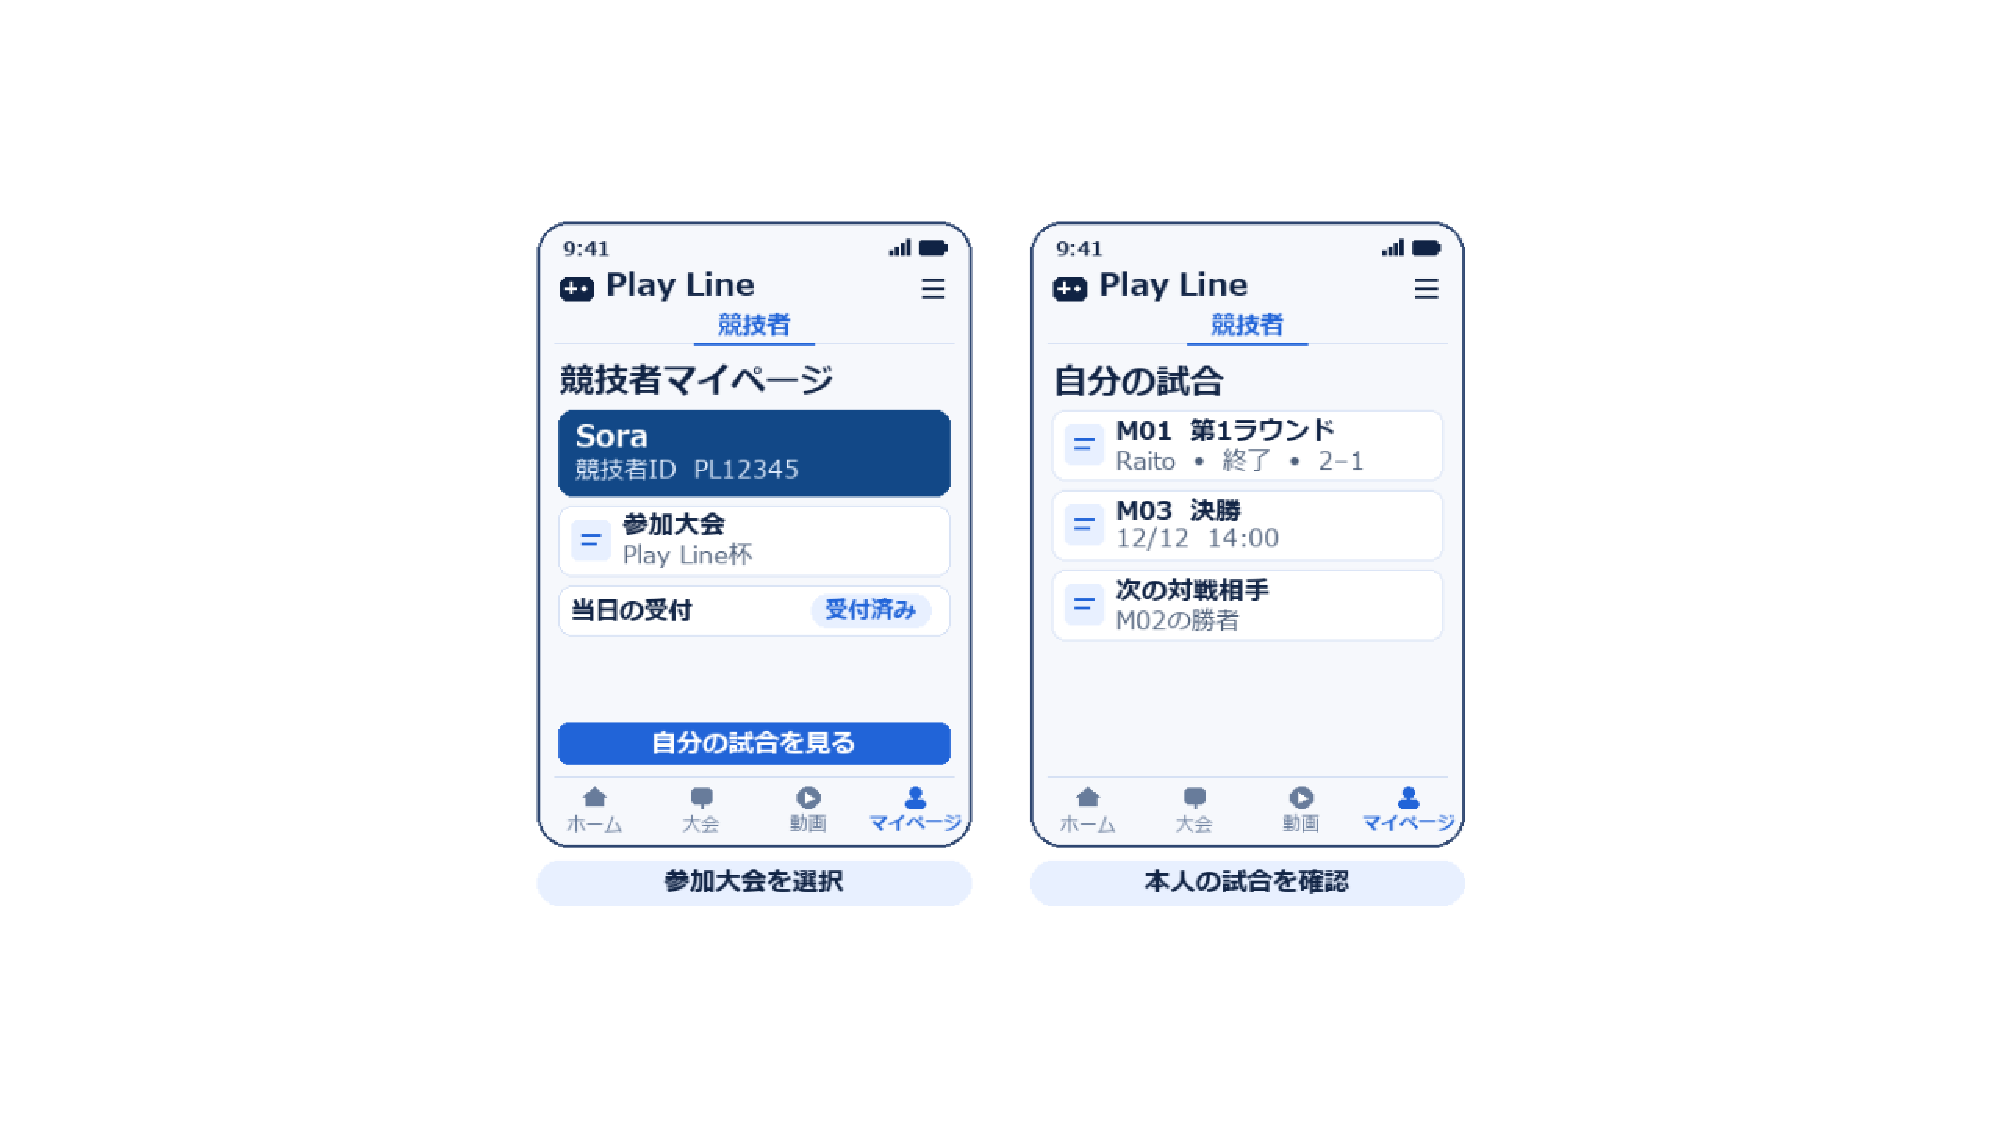
\includegraphics[width=\linewidth]{figures/03/3-2_mypage.pdf}
    \caption{競技者マイページ・試合情報画面イメージ}
    \label{fig:player_mypage_ui}
\end{figure}

\subsection{トーナメント・試合管理サブシステム}
大会形式に応じた対戦組み合わせを作成し、試合結果に基づいて大会の進行状況を管理する。

\subsubsection*{(a) トーナメント作成機能}
\begin{description}
    \item[入力：]大会ID、競技者情報、大会形式
    \item[出力：]トーナメント情報、試合組み合わせ
    \item[処理：]競技者情報を取得し、シングルエリミネーションまたは総当たり方式の
                対戦組み合わせを生成する。作成後、主催者が内容を確認する。
\end{description}

\begin{figure}[H]
    \centering
    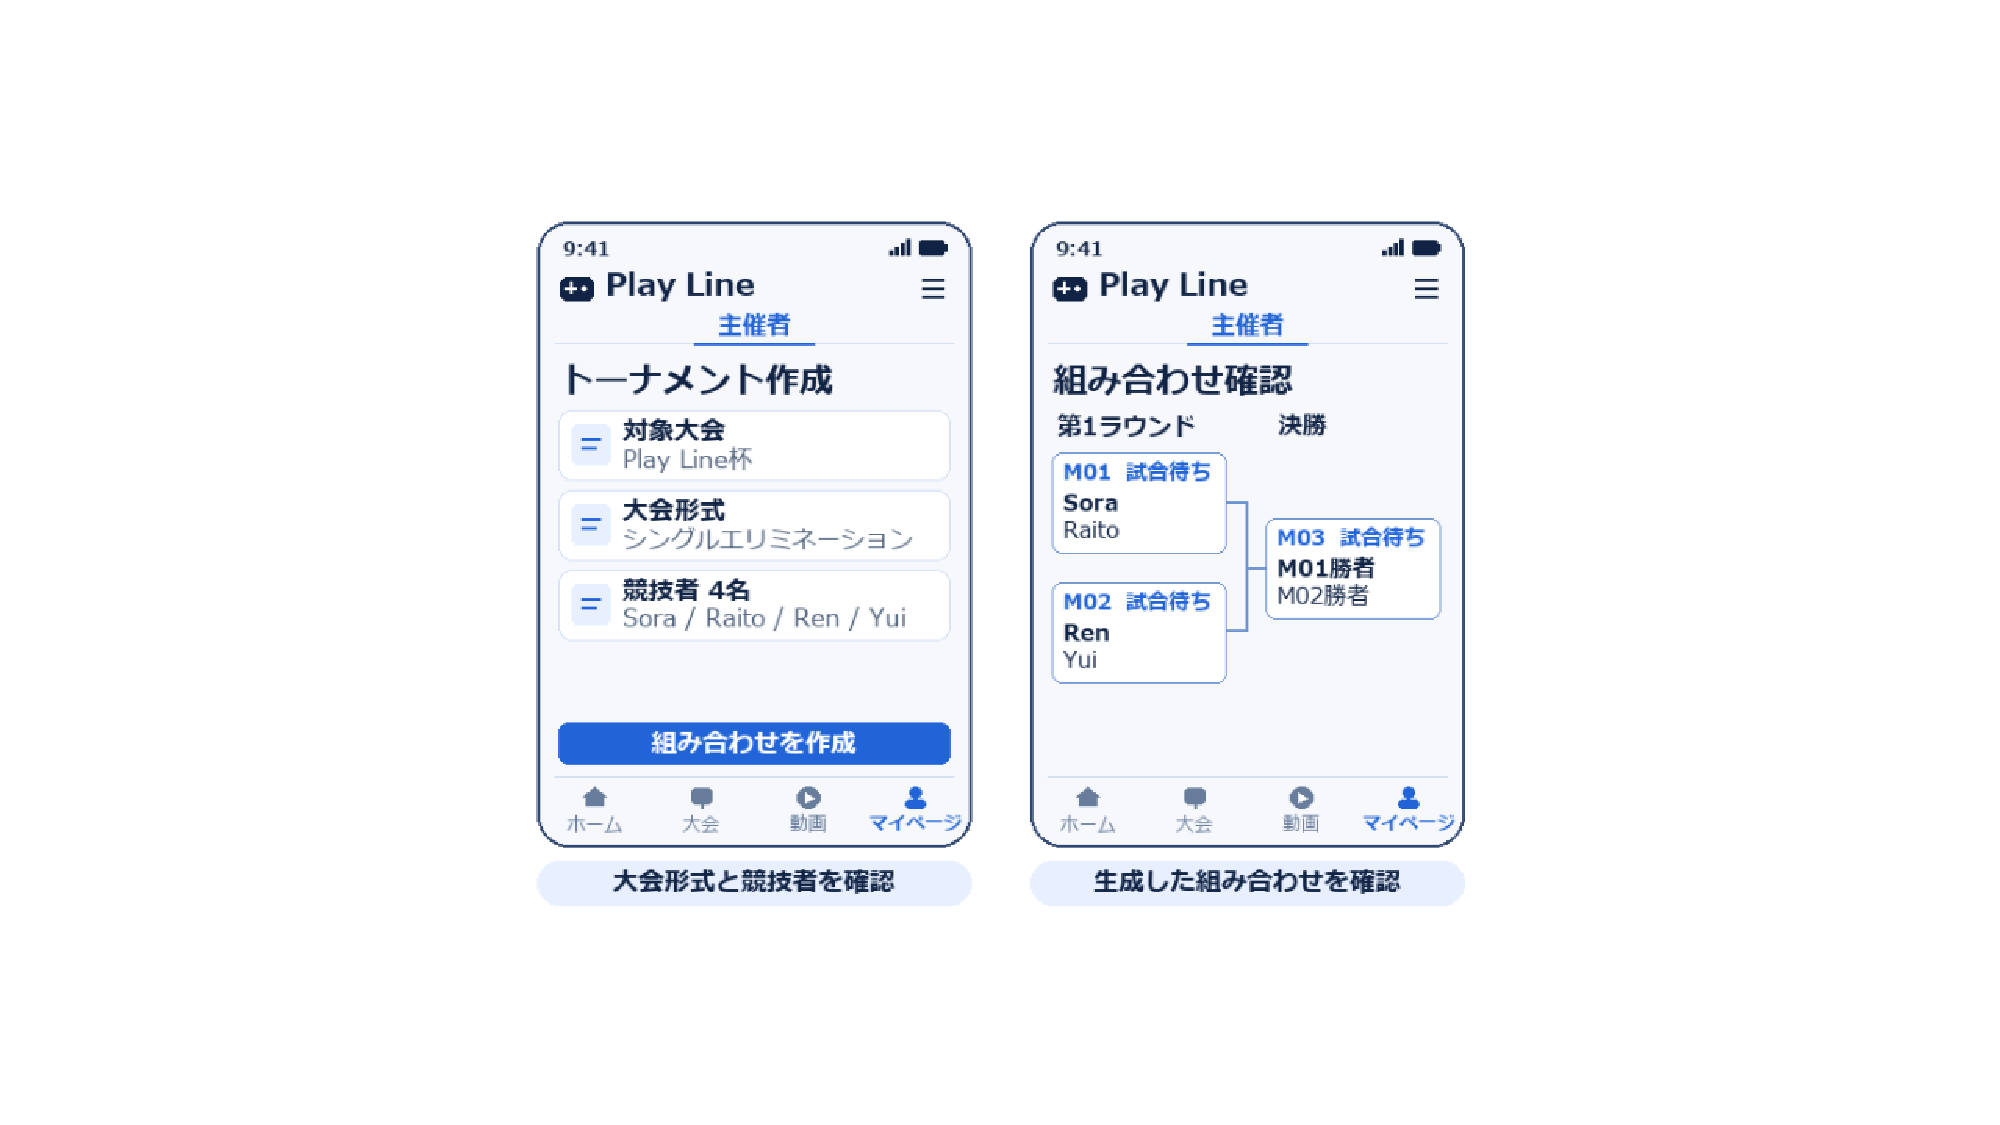
\includegraphics[width=\linewidth]{figures/03/3-3_bracket.pdf}
    \caption{トーナメント作成画面イメージ}
    \label{fig:tournament_bracket_ui}
\end{figure}

\subsubsection*{(b) 試合結果登録機能}
\begin{description}
    \item[入力：]試合ID、競技者ごとの得点・勝敗等
    \item[出力：]試合結果、登録・確認状態
    \item[処理：]試合終了後、競技者が結果を入力し、対戦相手が入力内容を確認する。
                両者の確認が一致した場合に結果を確定する。
                主催者は不一致や未確認の場合に内容を確認・修正でき、
                必要に応じて直接結果を登録する。
\end{description}

\begin{figure}[H]
    \centering
    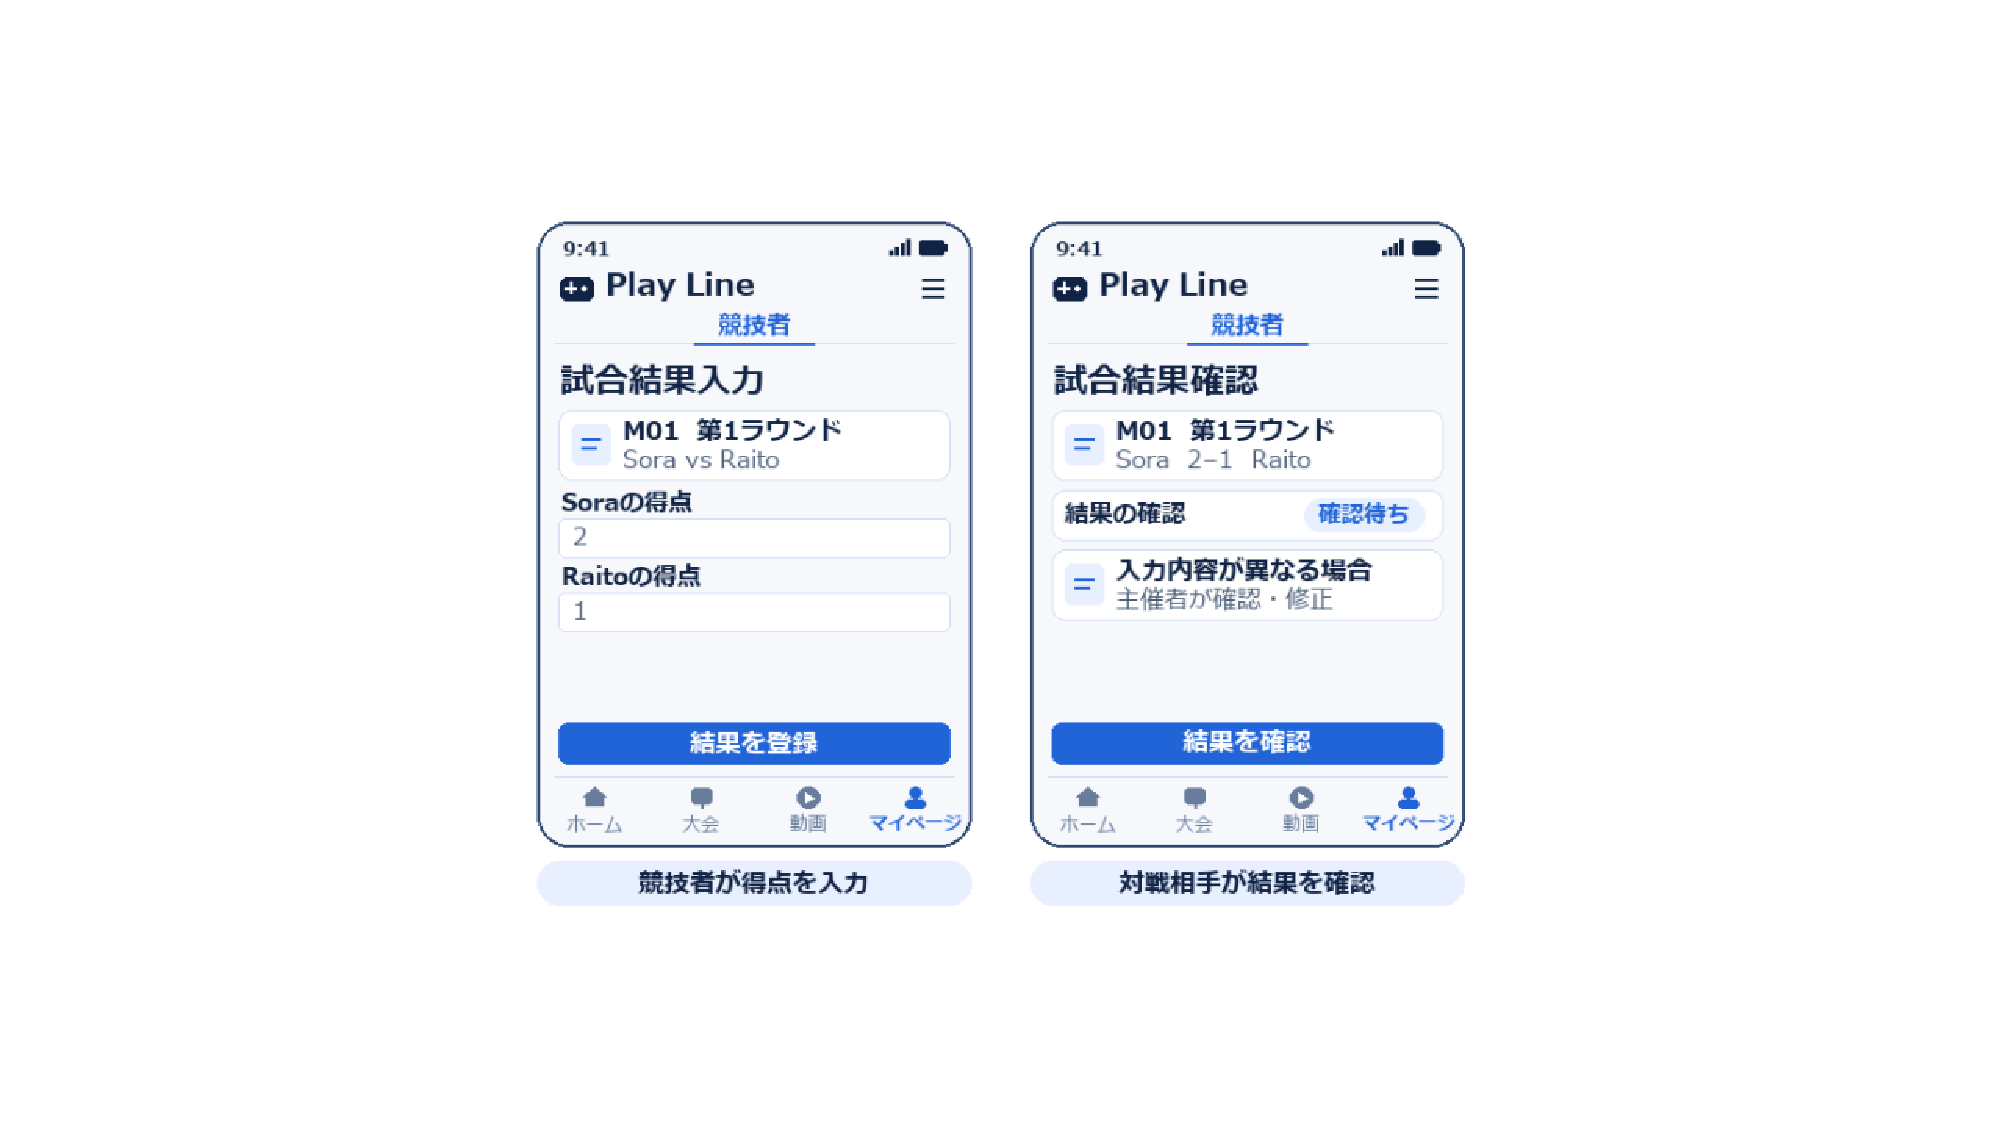
\includegraphics[width=\linewidth]{figures/03/3-3_result.pdf}
    \caption{試合結果登録画面イメージ}
    \label{fig:match_result_ui}
\end{figure}

\subsubsection*{(c) 大会進行更新機能}
\begin{description}
    \item[入力：]確定した試合結果
    \item[出力：]次ラウンドの対戦情報、順位、更新後の進行状況
    \item[処理：]シングルエリミネーションでは勝者を次のラウンドに割り当てる。
                総当たり方式では勝利数などを集計し、順位表を更新する。
\end{description}

\begin{figure}[H]
    \centering
    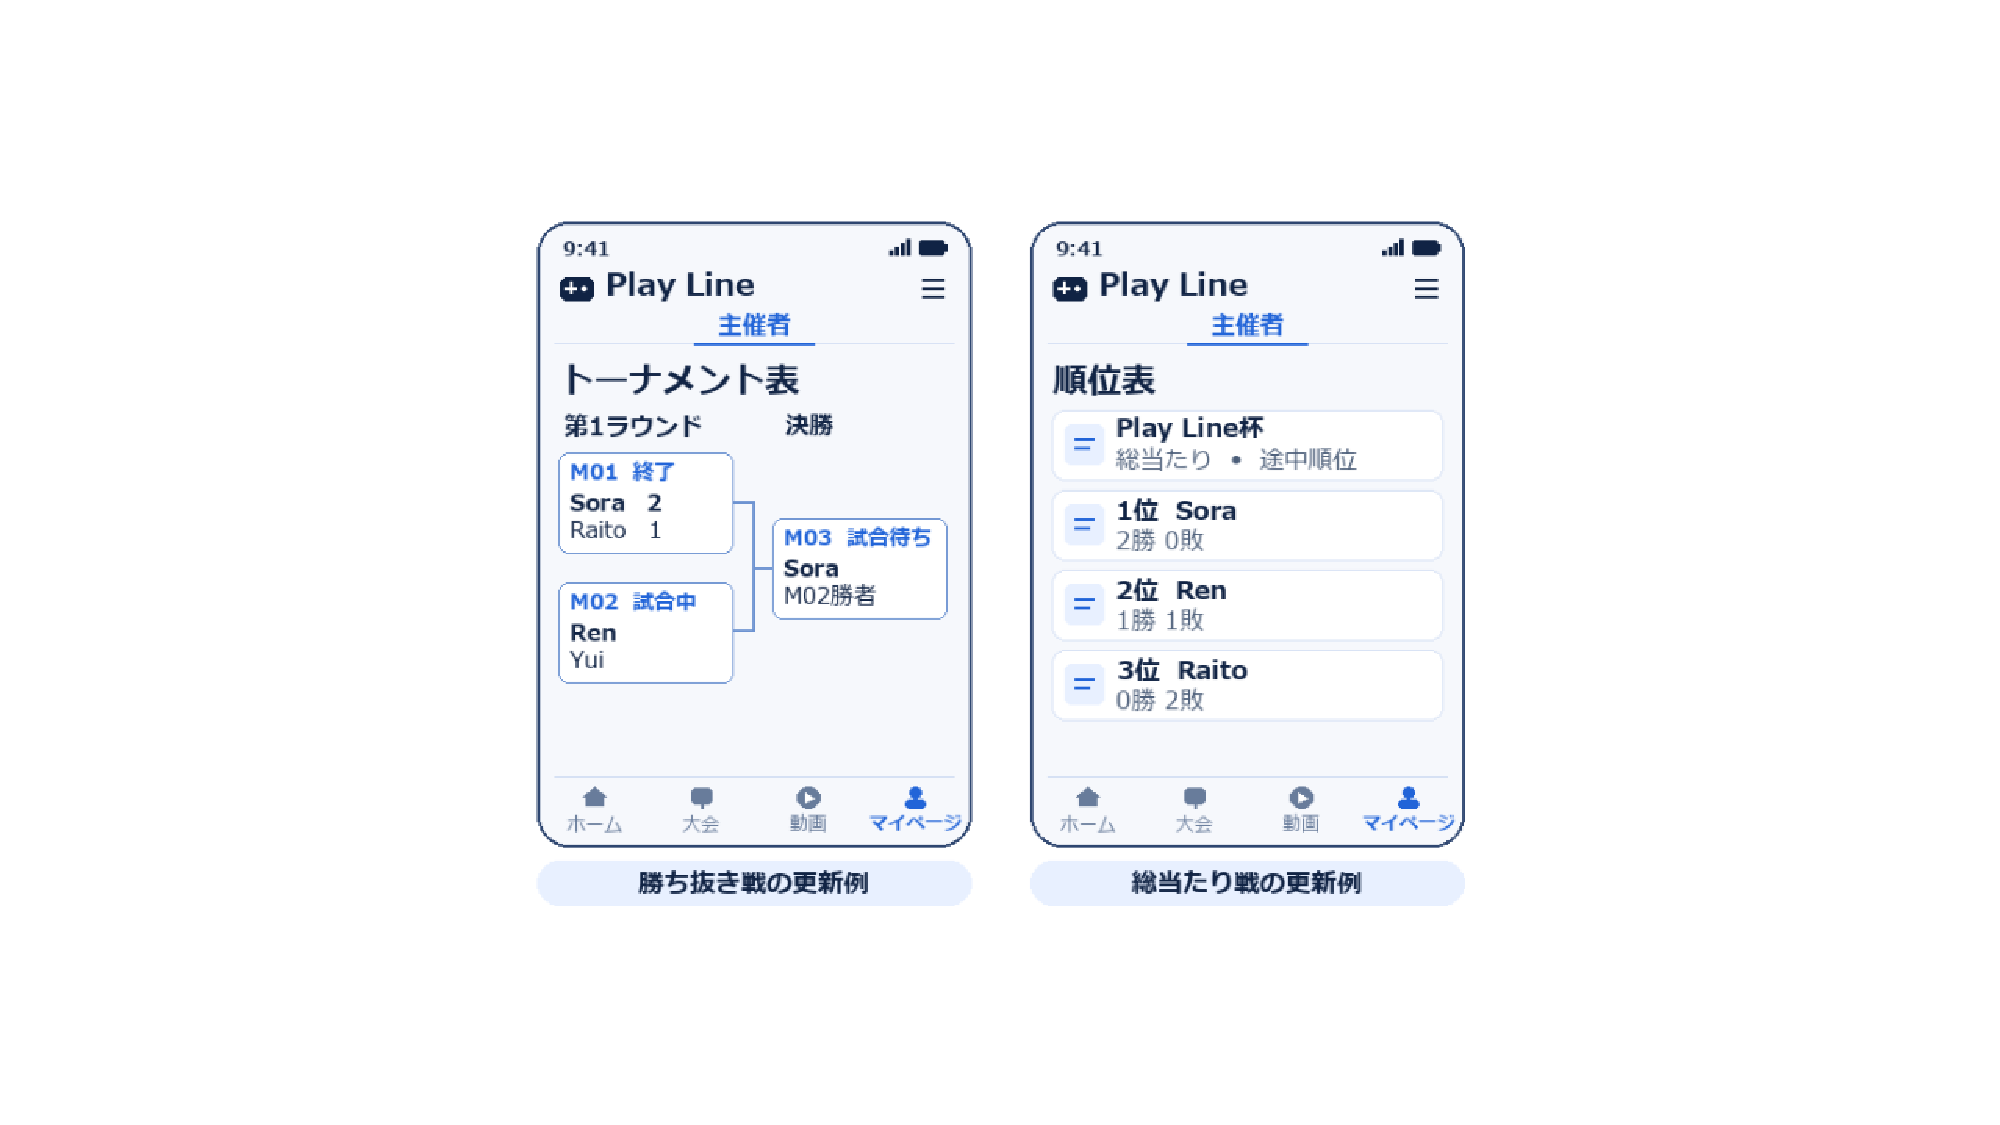
\includegraphics[width=\linewidth]{figures/03/3-3_progress.pdf}
    \caption{大会進行状況・対戦表画面イメージ}
    \label{fig:tournament_progress_ui}
\end{figure}

\subsubsection*{(d) 試合状態管理機能}
\begin{description}
    \item[入力：]試合ID、試合状態
    \item[出力：]試合中・試合待ち・試合終了等の状態
    \item[処理：]各試合の状態を管理し、大会ページおよび選手ページに反映する。
                具体的な状態遷移条件は内部設計で定義する。
\end{description}

\begin{figure}[H]
    \centering
    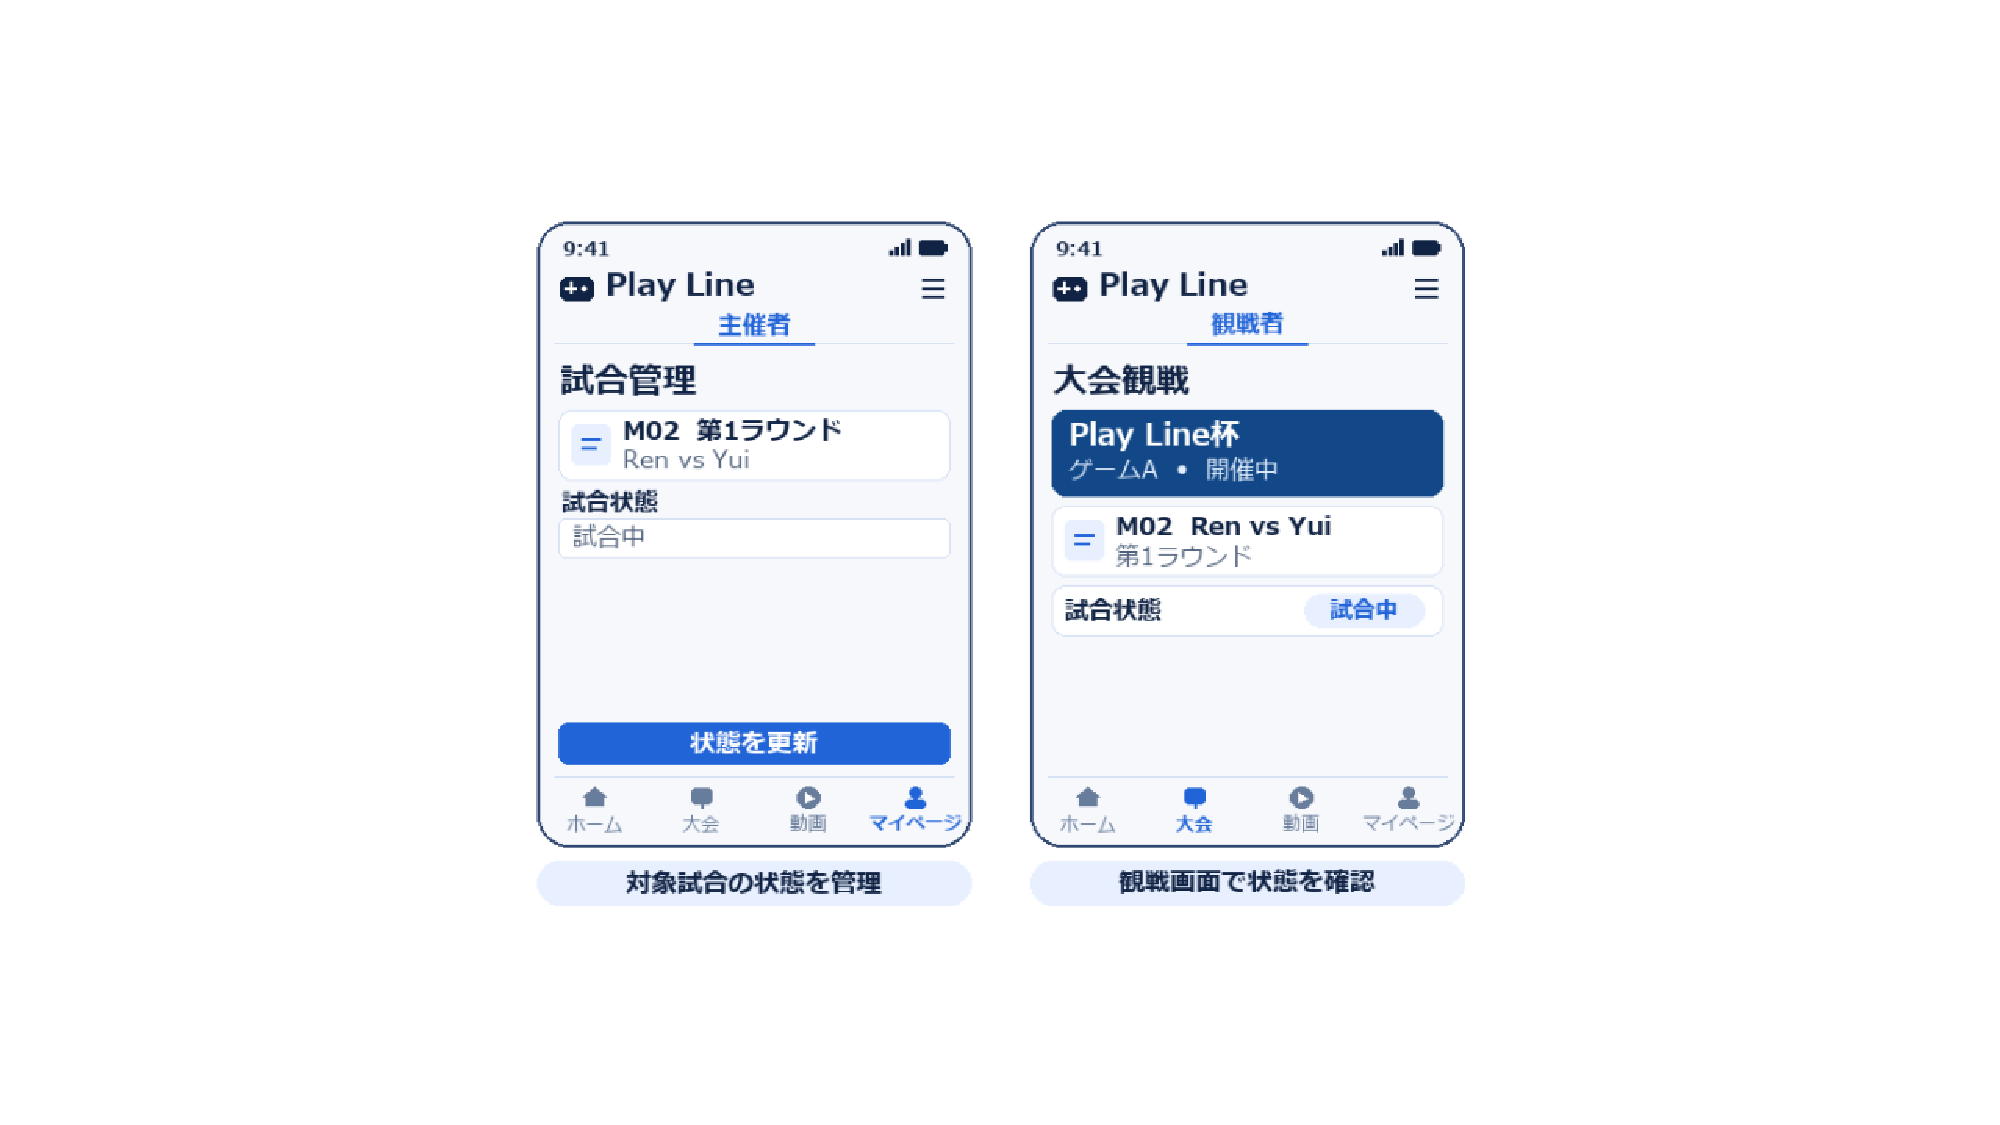
\includegraphics[width=\linewidth]{figures/03/3-3_status.pdf}
    \caption{試合状態管理画面イメージ}
    \label{fig:match_status_ui}
\end{figure}

\subsubsection*{(e) 試合配信情報管理機能}
\begin{description}
    \item[入力：]試合ID、配信URL
    \item[出力：]試合に紐づけられた配信情報、配信状態
    \item[処理：]主催者が試合ごとの配信URLを登録し、対象となる試合情報と関連付けて保存する。
                登録された配信情報は大会観戦画面および選手詳細画面に提供する。
                配信情報の取得方法や更新条件は内部設計で定義する。
\end{description}

\begin{figure}[H]
    \centering
    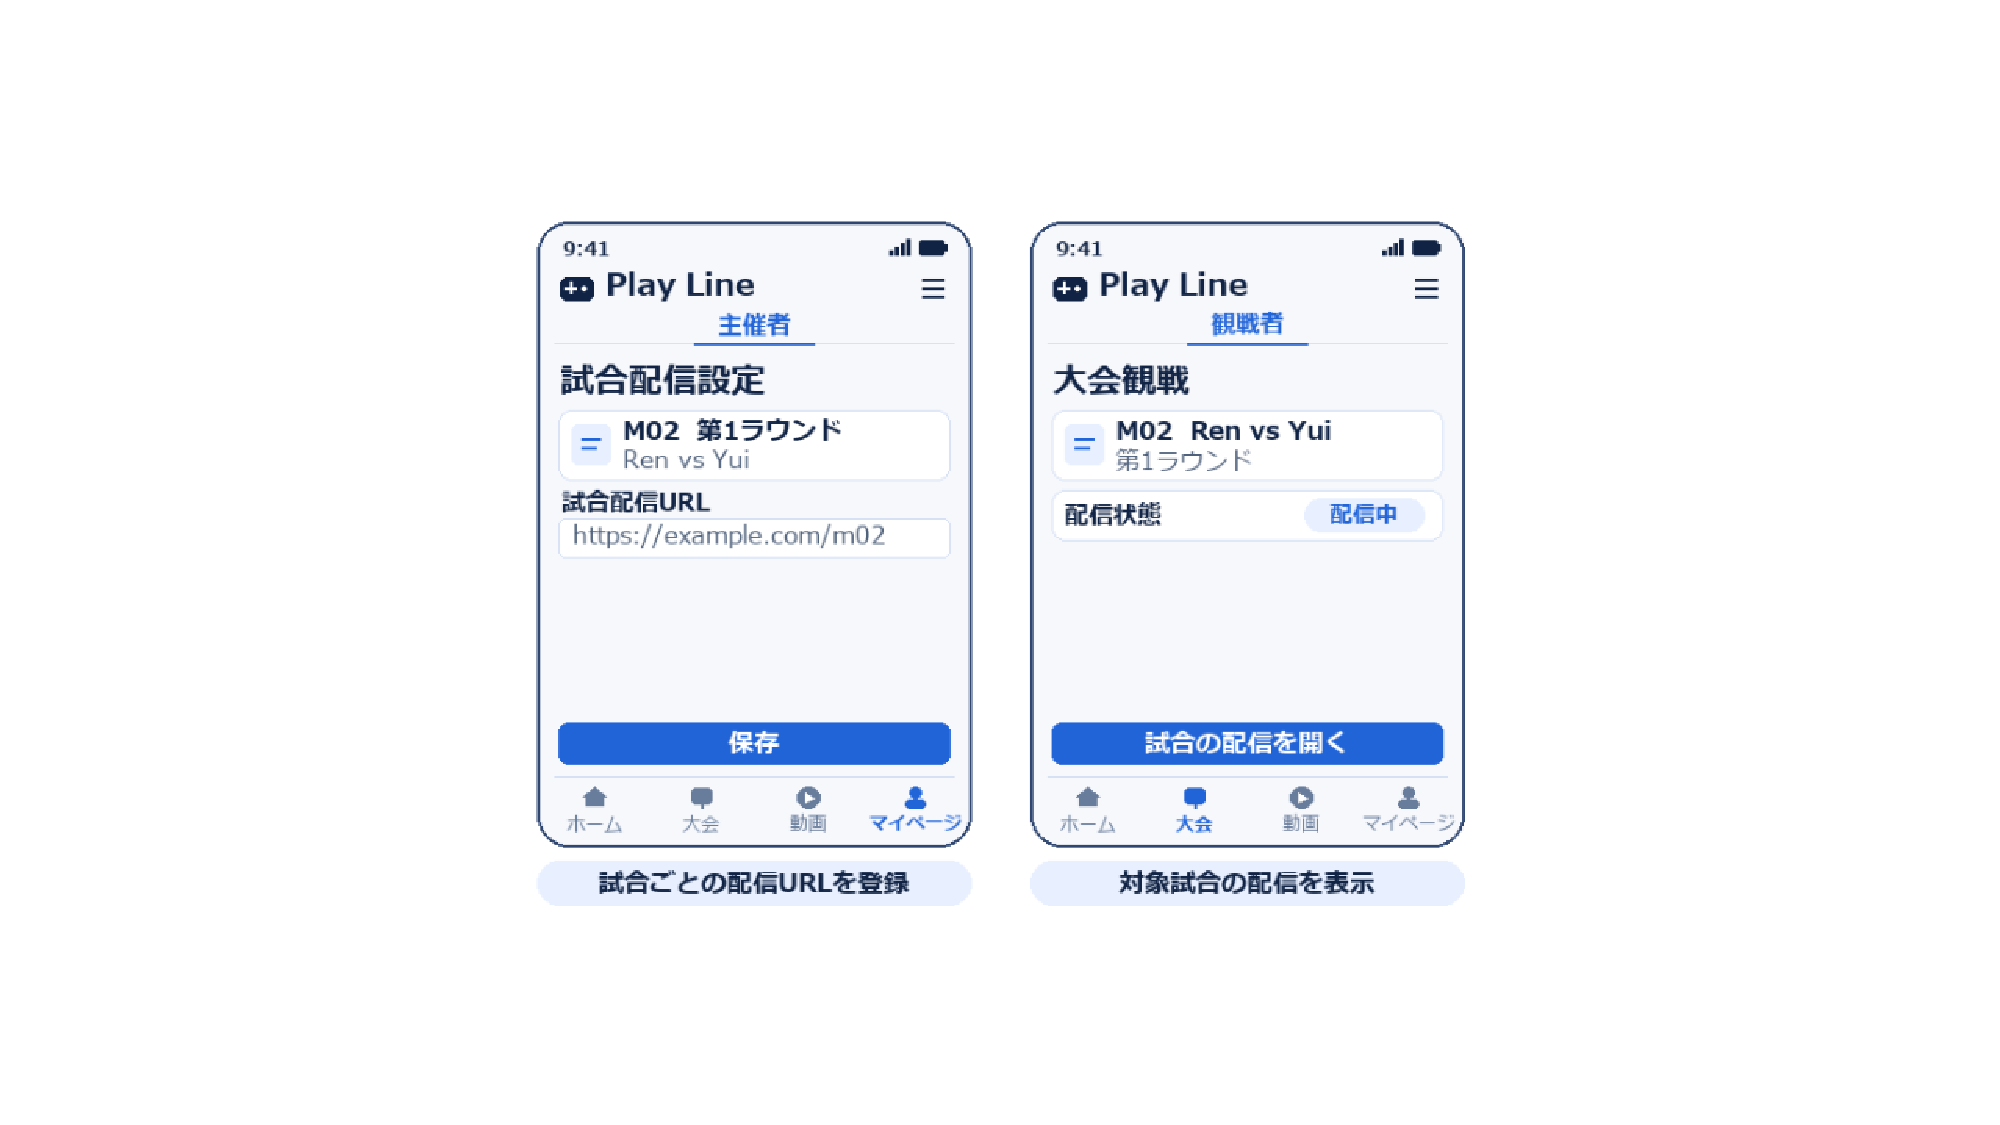
\includegraphics[width=\linewidth]{figures/03/3-3_stream.pdf}
    \caption{試合配信情報管理画面イメージ}
    \label{fig:match_stream_ui}
\end{figure}

\subsection{観戦者向け情報提供サブシステム}
観戦者が大会全体の状況と関心のある選手の情報をまとめて確認できるようにする。

\subsubsection*{(a) 選手検索・選手情報表示機能}
\begin{description}
    \item[入力：]プレイヤー名等の検索条件、選手ID
    \item[出力：]選手プロフィール、大会参加履歴、成績
    \item[処理：]登録されている選手を検索し、選手を識別する固定IDに関連付けられた情報を表示する。
                プレイヤー名が変更されても同一選手として追跡できるようにする。
\end{description}

\begin{figure}[H]
    \centering
    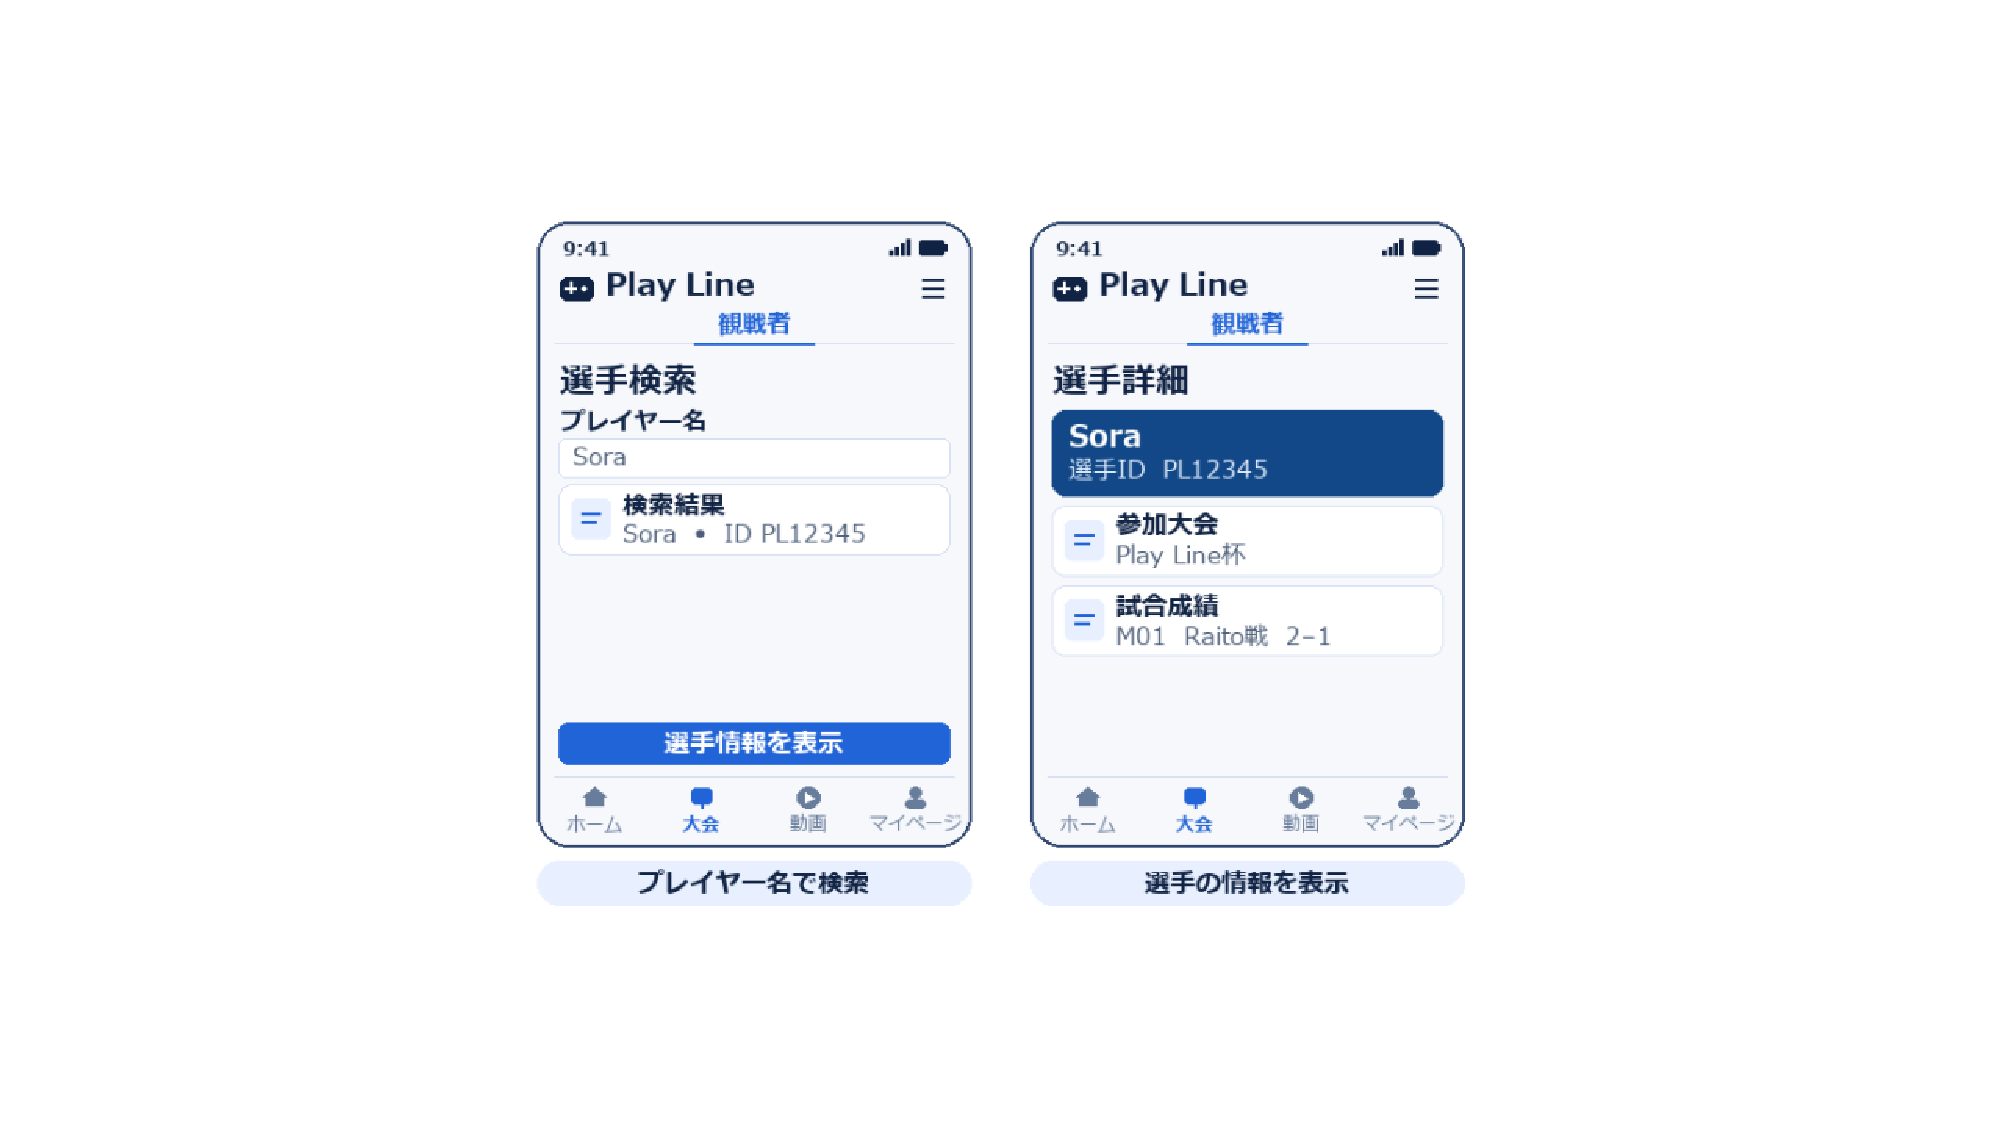
\includegraphics[width=\linewidth]{figures/03/3-4_player.pdf}
    \caption{選手検索・プロフィール画面イメージ}
    \label{fig:spectator_player_ui}
\end{figure}

\subsubsection*{(b) お気に入り選手登録機能}
\begin{description}
    \item[入力：]観戦者の利用者情報、選手ID
    \item[出力：]お気に入り選手一覧
    \item[処理：]観戦者が選択した選手IDをお気に入り情報として保存し、
                次回以降の選手情報表示に利用する。
\end{description}

\begin{figure}[H]
    \centering
    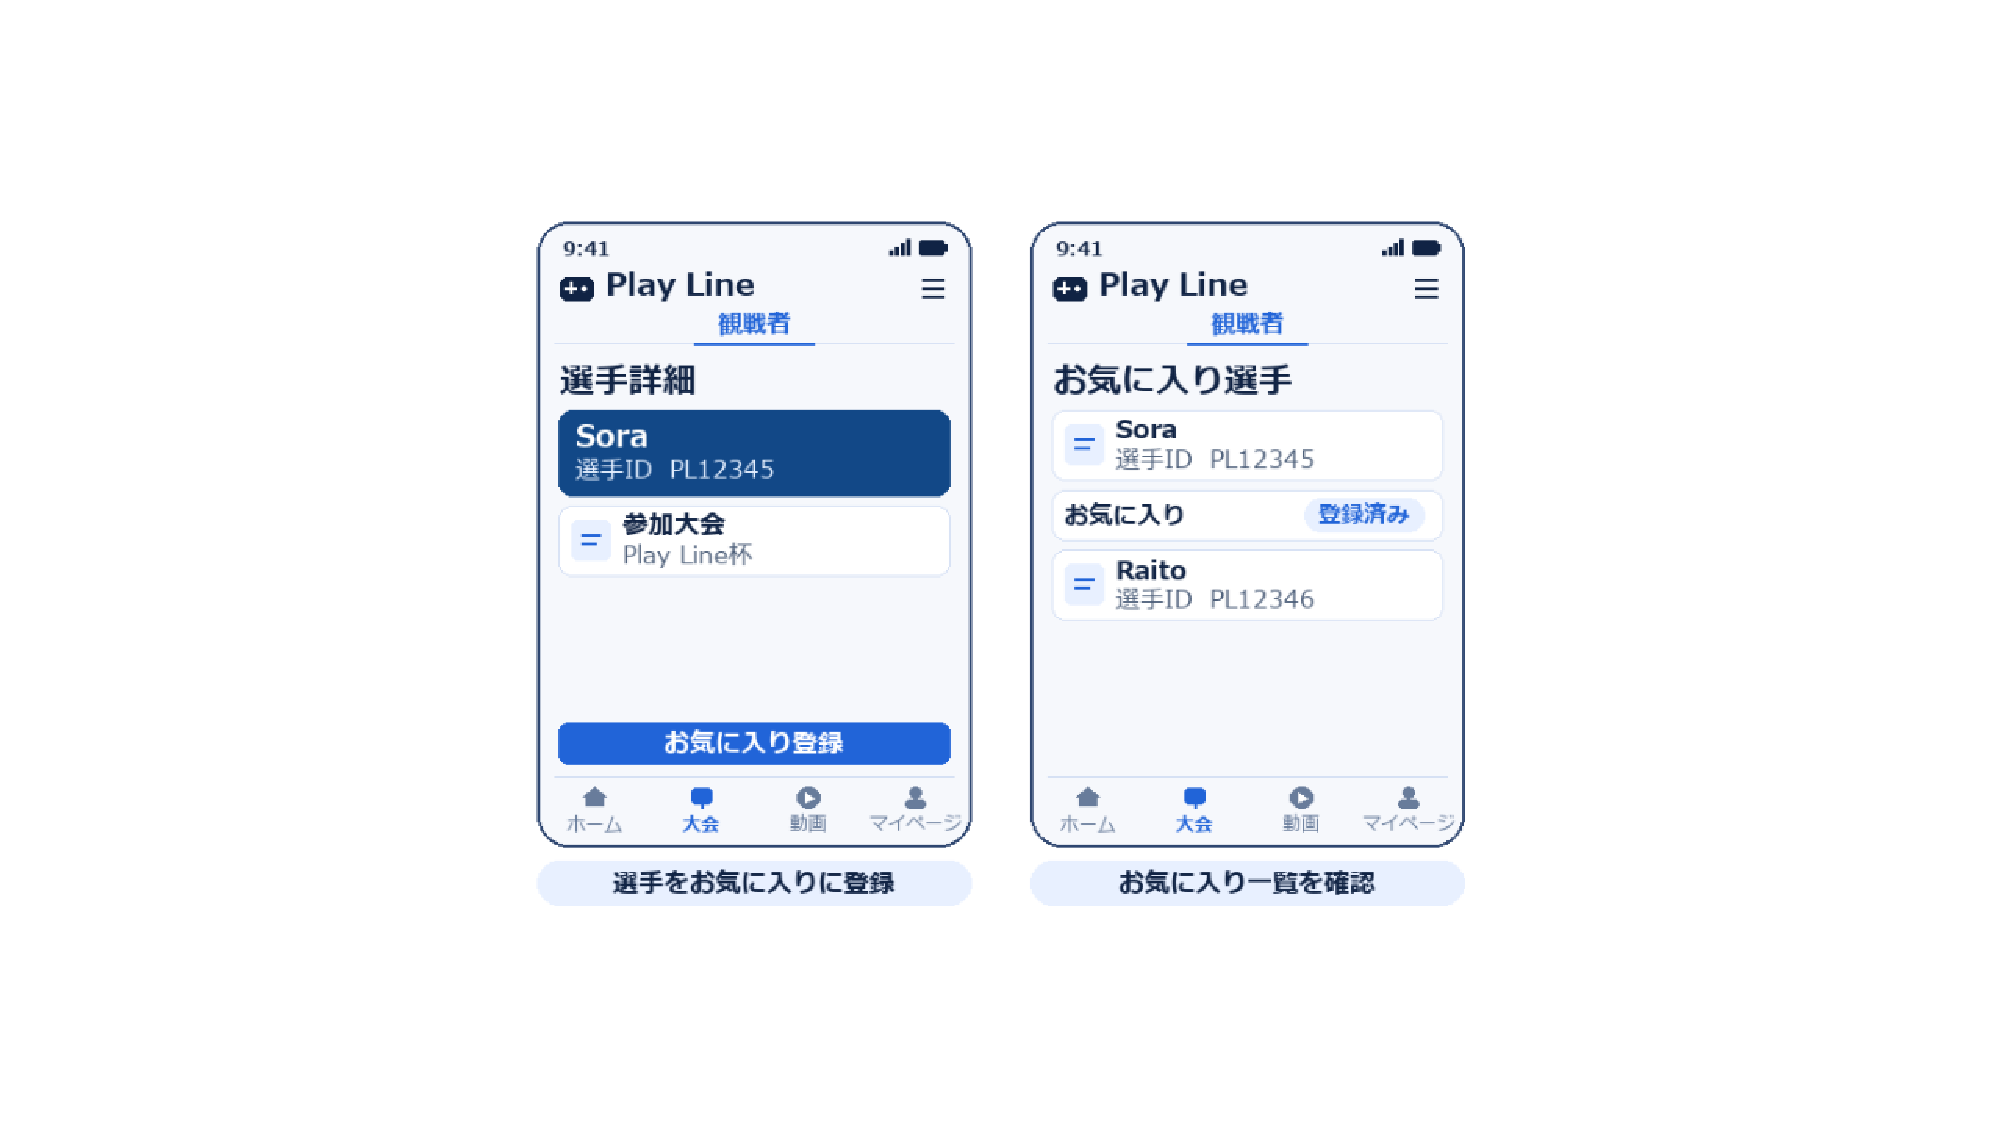
\includegraphics[width=\linewidth]{figures/03/3-4_favorite.pdf}
    \caption{お気に入り選手一覧画面イメージ}
    \label{fig:spectator_favorite_ui}
\end{figure}

\subsubsection*{(c) 注目選手追跡機能}
\begin{description}
    \item[入力：]選手ID、大会ID
    \item[出力：]現在の試合状況、過去の試合結果、次の対戦相手、トーナメント上の位置
    \item[処理：]選手に関連する試合情報と大会情報を取得し、選手単位でまとめて表示する。
                対戦相手が未確定の場合は未確定であることを表示する。
\end{description}

\begin{figure}[H]
    \centering
    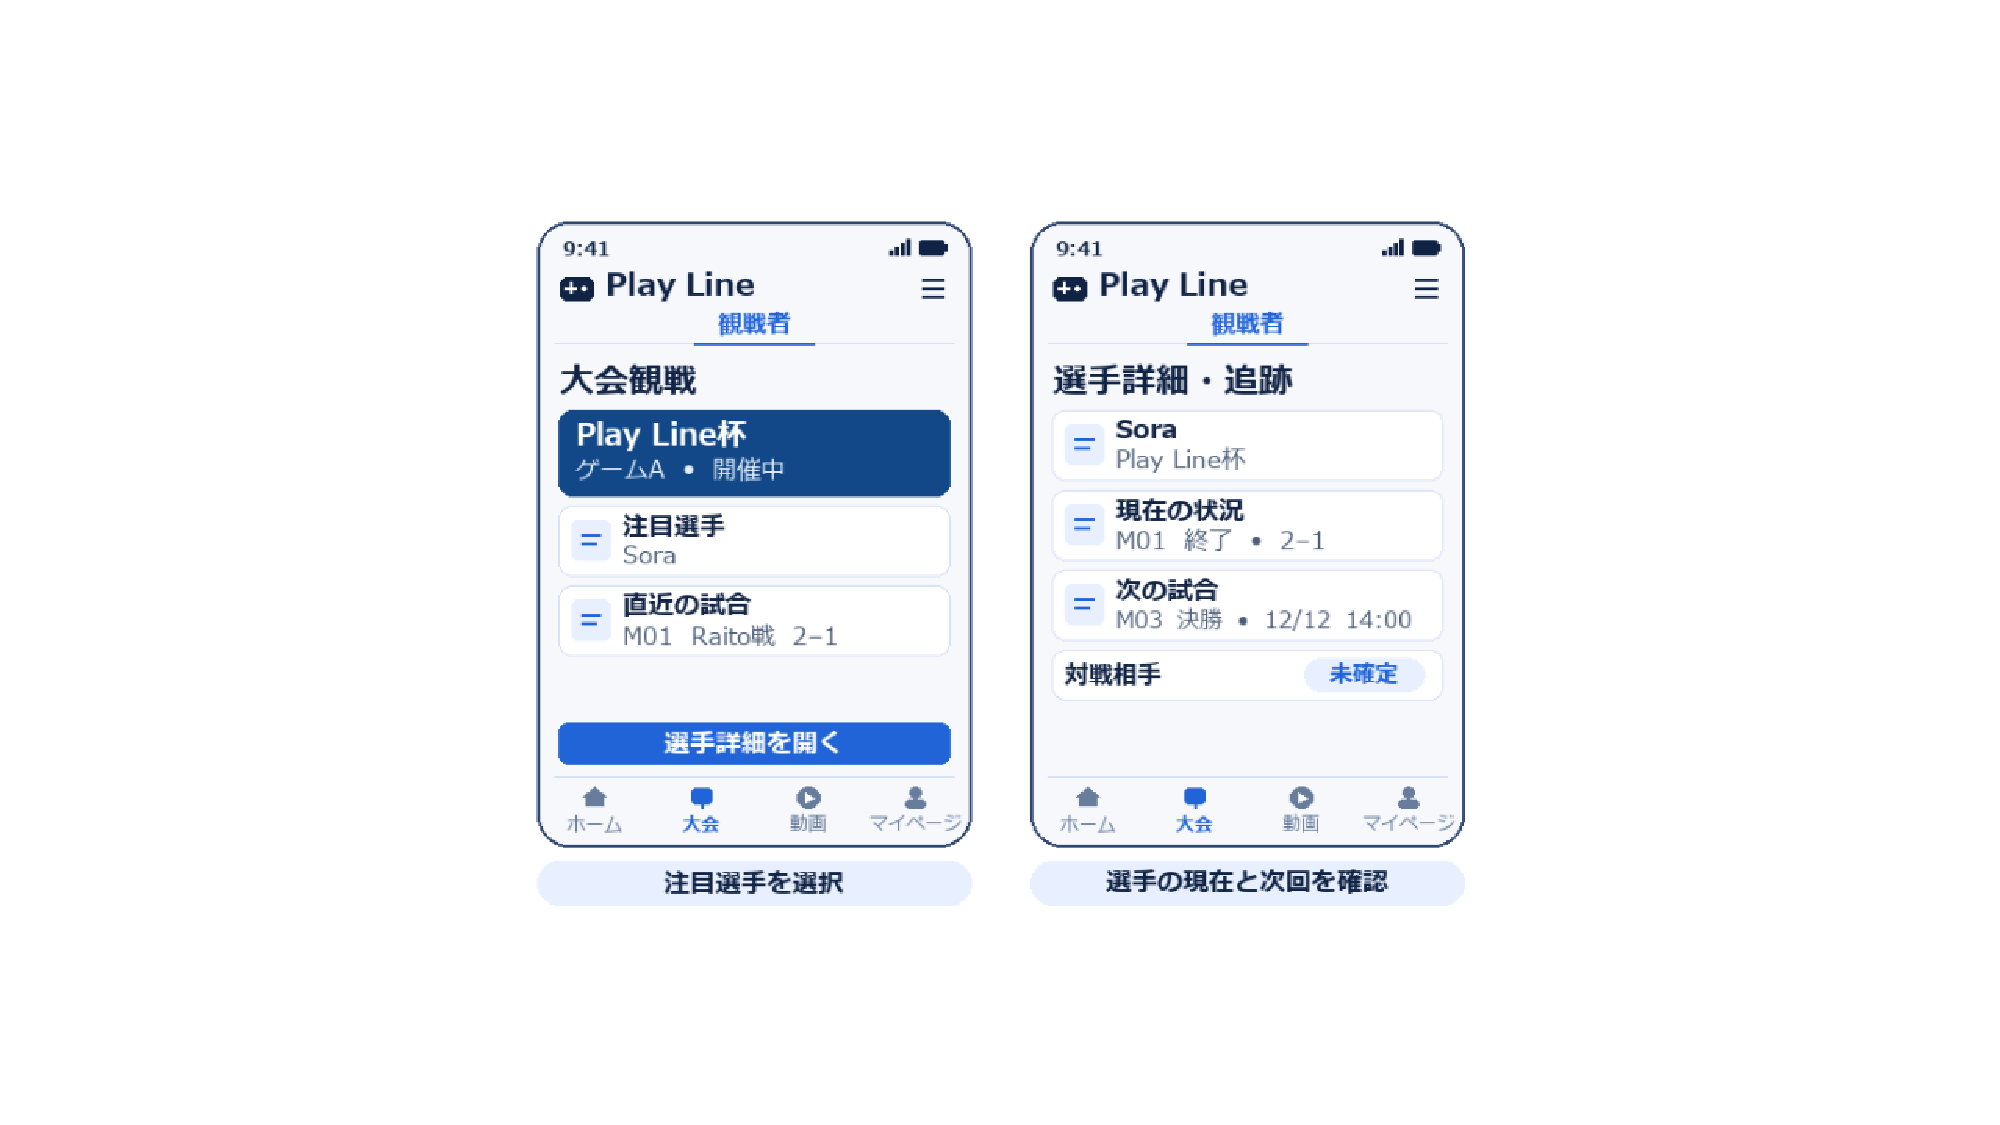
\includegraphics[width=\linewidth]{figures/03//3-4_tracking.pdf}
    \caption{注目選手追跡画面イメージ}
    \label{fig:spectator_tracking_ui}
\end{figure}

\subsubsection*{(d) 対戦履歴確認機能}
\begin{description}
    \item[入力：]選手ID、比較対象の選手ID
    \item[出力：]過去の対戦結果
    \item[処理：]指定した選手同士の過去の試合情報を検索して表示する。
\end{description}

\begin{figure}[H]
    \centering
    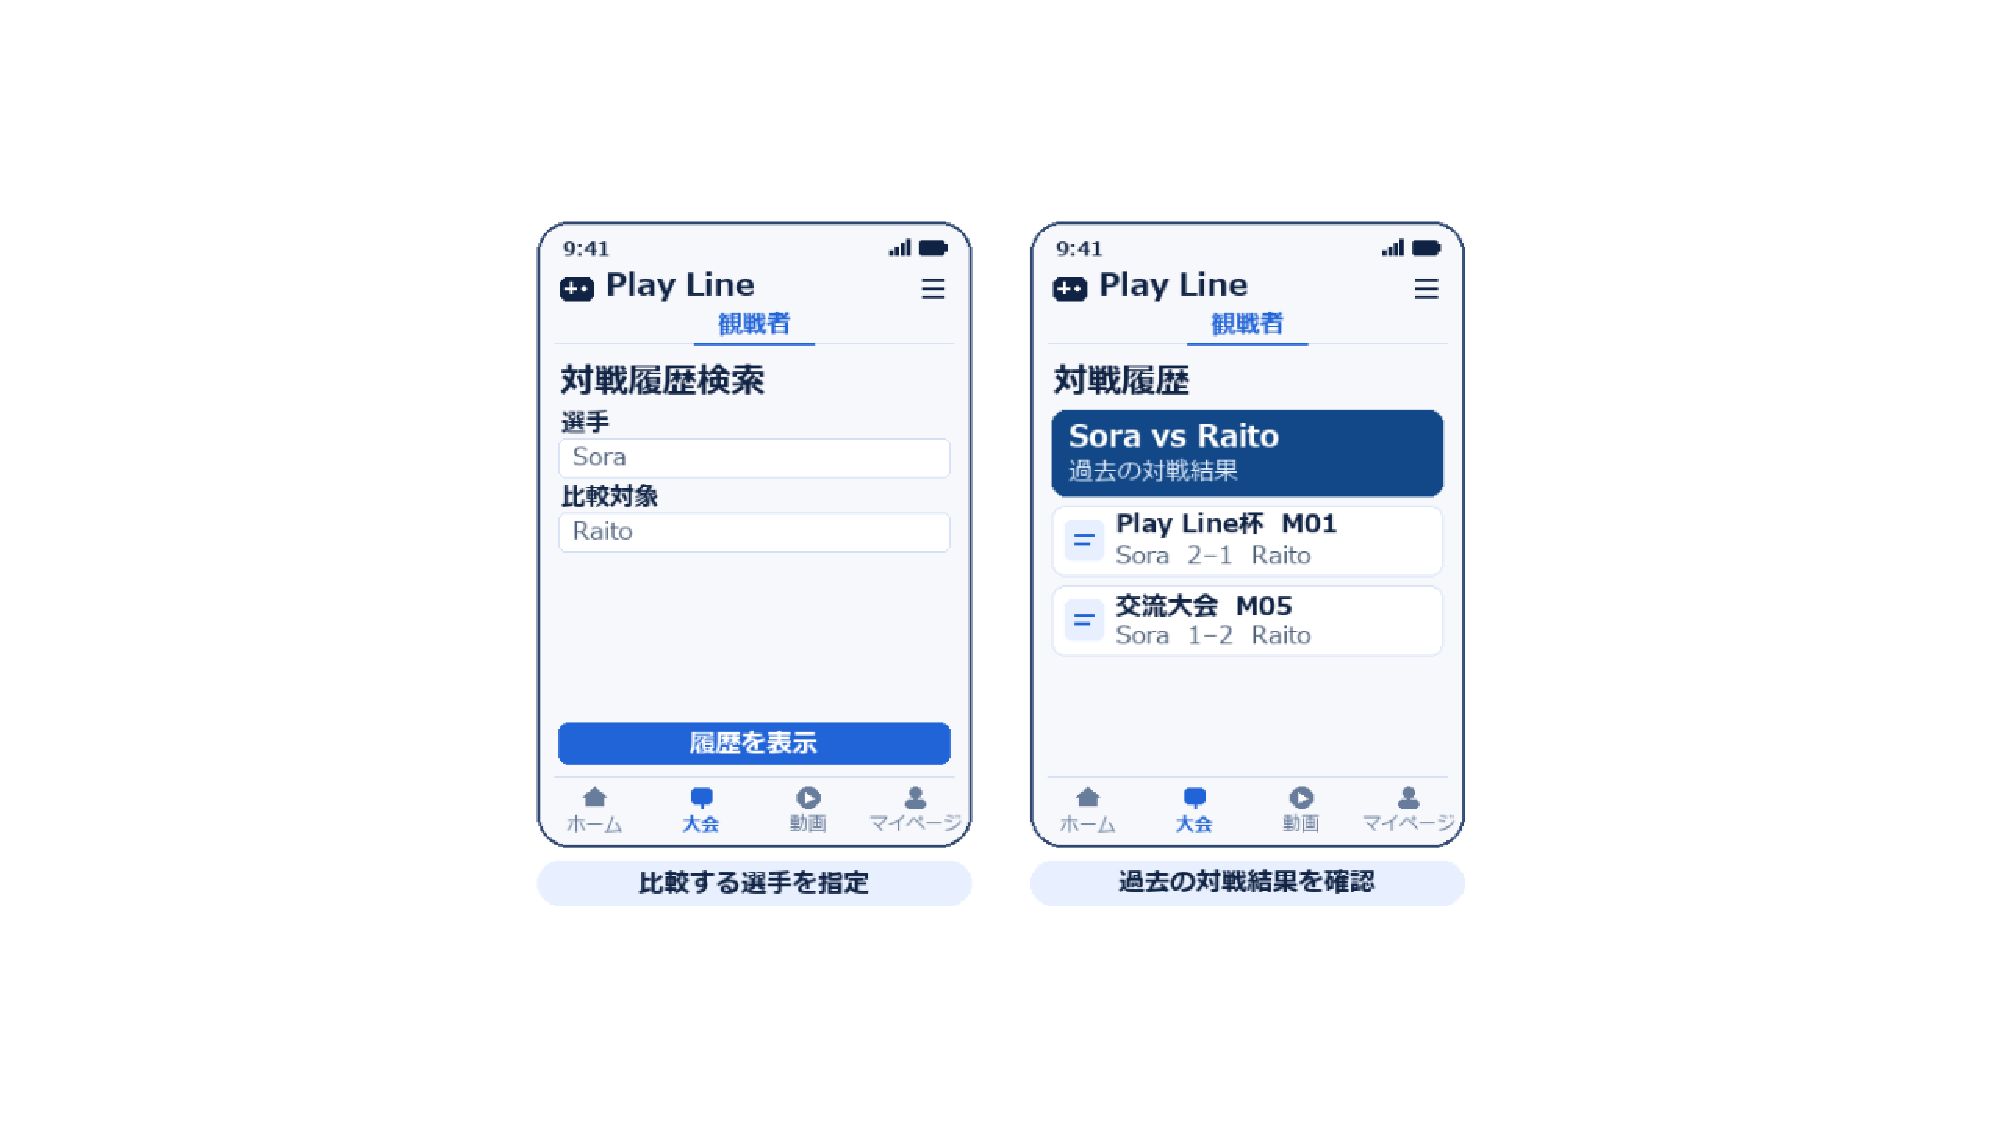
\includegraphics[width=\linewidth]{figures/03/3-4_matchup.pdf}
    \caption{対戦履歴確認画面イメージ}
    \label{fig:spectator_history_ui}
\end{figure}

\subsubsection*{(e) ライブ配信URL表示機能}
\begin{description}
    \item[入力：]大会ID、主催者が登録したライブ配信URL
    \item[出力：]配信ページへのリンク
    \item[処理：]大会情報に登録された外部配信URLを大会ページに表示し、
                観戦者が外部サービスへアクセスできるようにする。
                映像配信ぞのものは本システムでは行わない。
\end{description}

\begin{figure}[H]
    \centering
    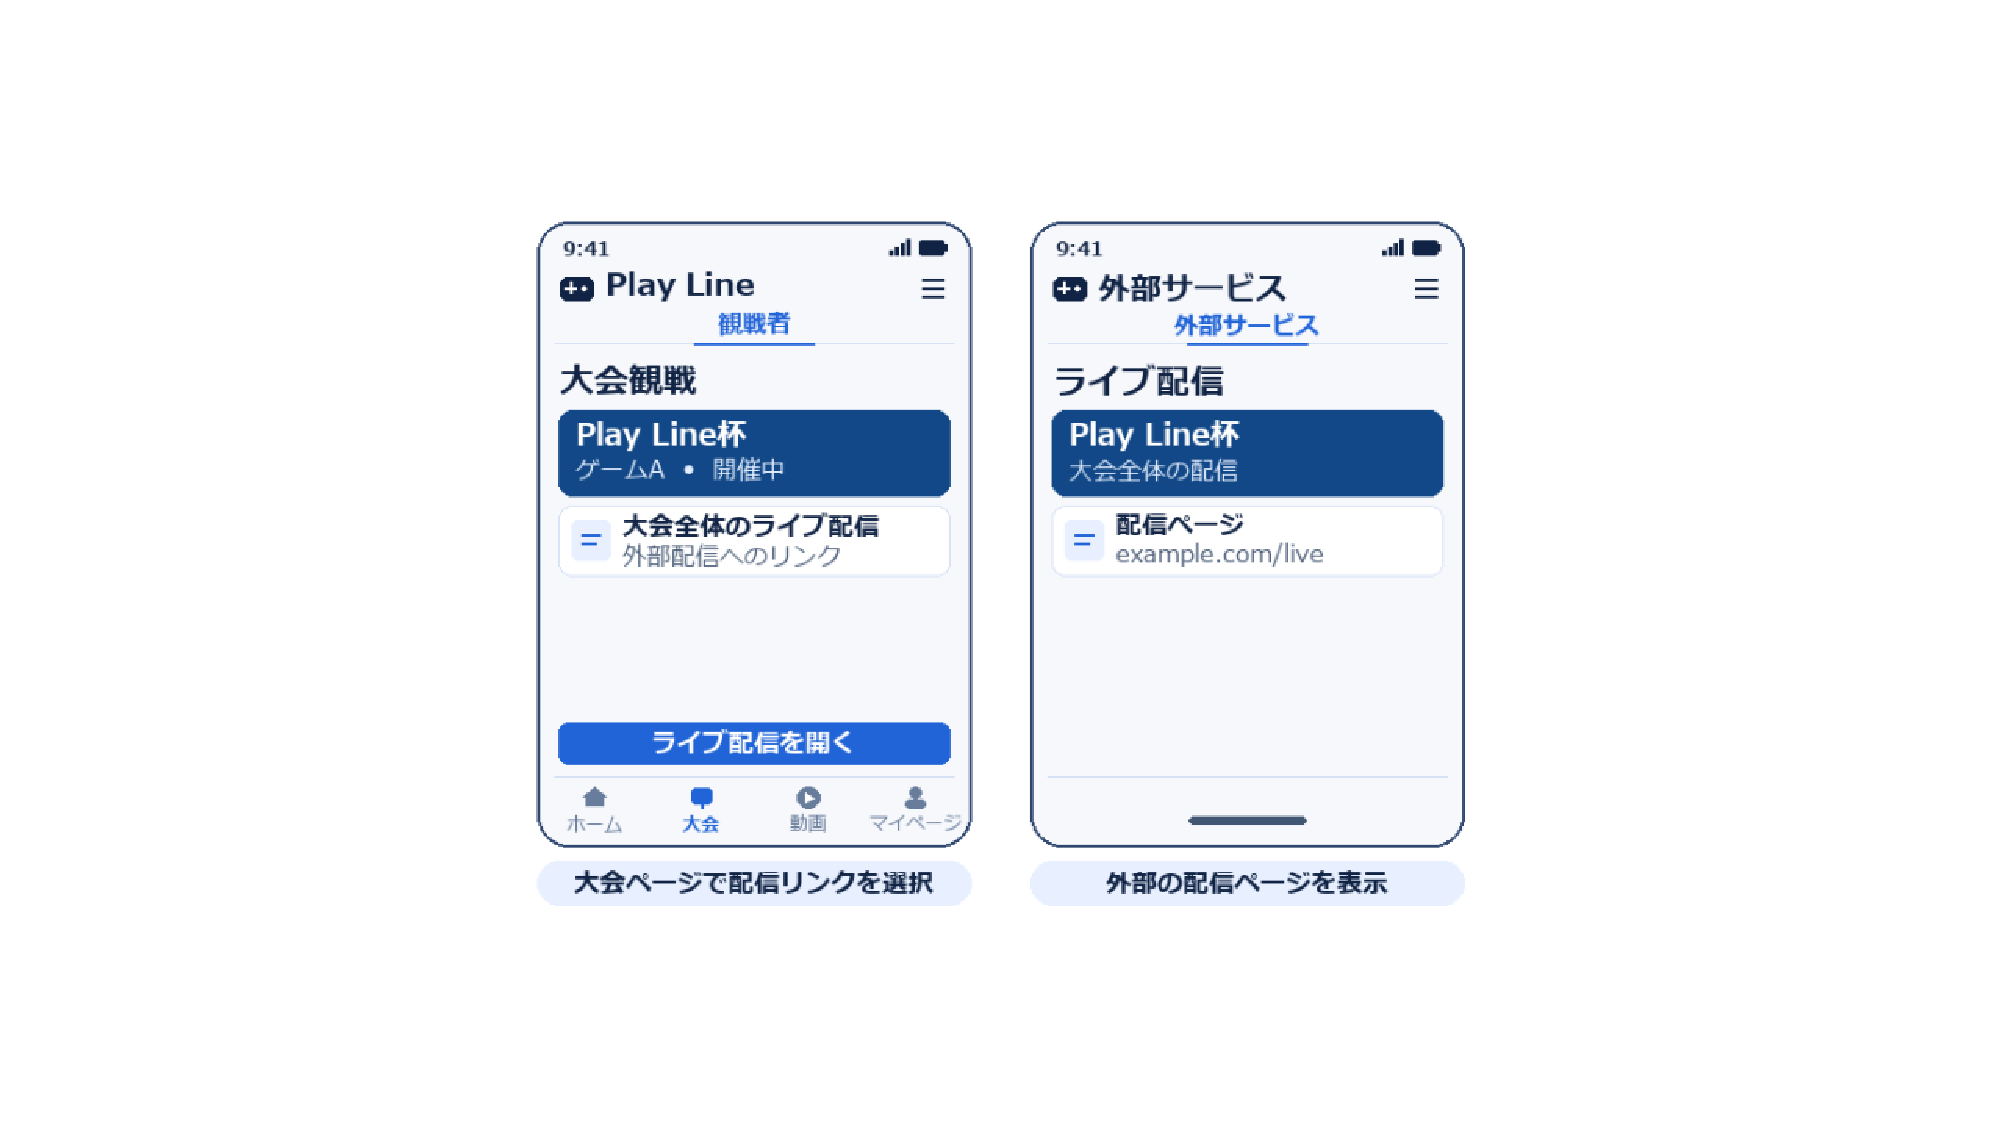
\includegraphics[width=\linewidth]{figures/03/3-4_stream.pdf}
    \caption{ライブ配信リンク表示画面イメージ}
    \label{fig:spectator_stream_ui}
\end{figure}

\subsubsection*{(f) 短尺動画閲覧機能}
\begin{description}
    \item[入力：]動画ジャンル、選択した動画
    \item[出力：]ジャンル別の短尺動画一覧、選択した動画の視聴リンク
    \item[処理：]初期画面の「人気のクリップ」や「動画」から動画一覧を開く。
                対戦ハイライト、攻略・解説、選手紹介などのジャンルで絞り込み、
                タイトルと再生時間を表示する。
                動画を選ぶと、外部の動画サービスで視聴できる。
\end{description}

\begin{figure}[H]
    \centering
    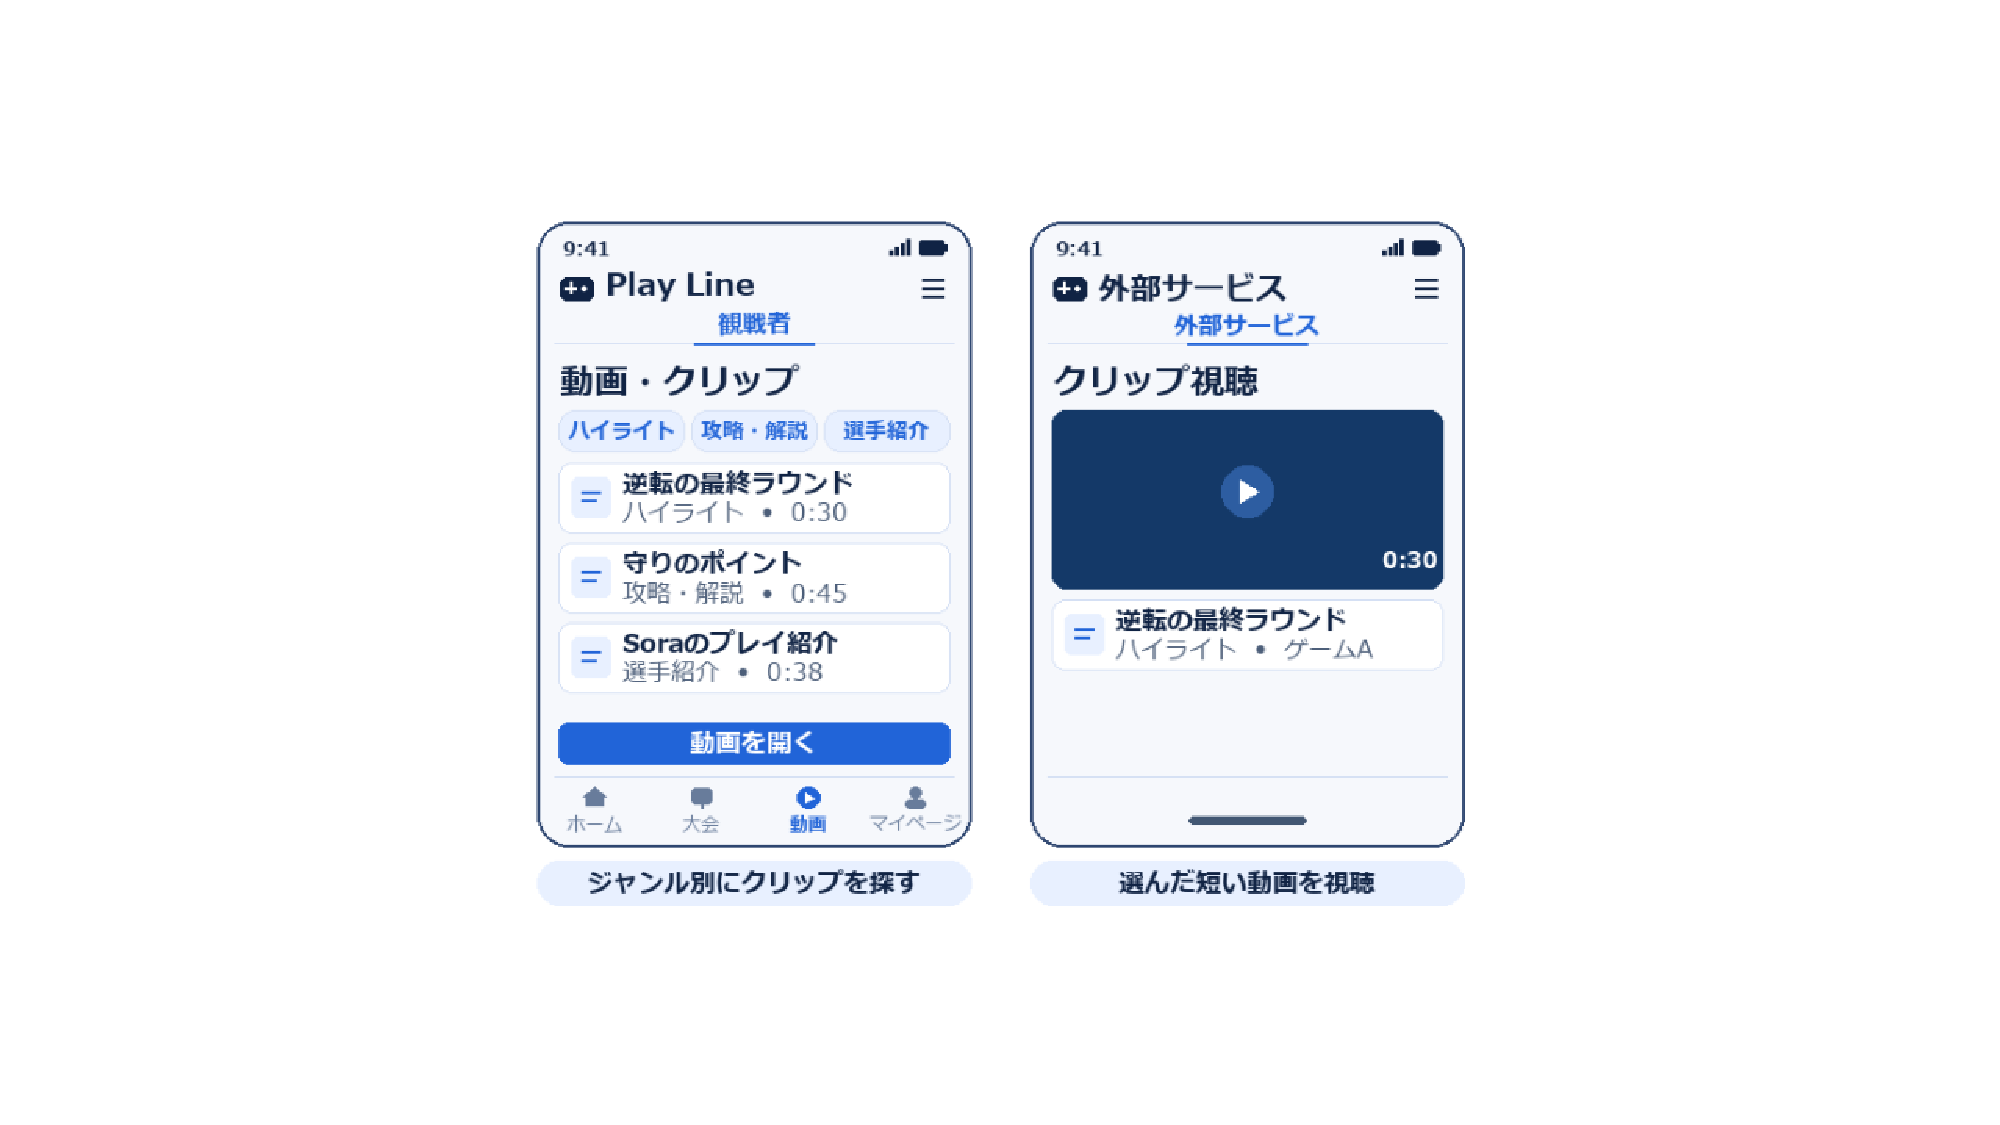
\includegraphics[width=\linewidth]{figures/03/3-4_video.pdf}
    \caption{短尺動画一覧・再生画面イメージ}
    \label{fig:spectator_video_ui}
\end{figure}

\subsection{通知サブシステム}

\subsubsection*{(a) メール通知機能}
\begin{description}
    \item[入力：]通知対象者のメールアドレス、通知内容、対象大会・試合情報
    \item[出力：]メール通知
    \item[処理：]試合予定の変更や試合結果の更新など、利用者に知らせる情報をメールで送信する。
                通知対象や送信タイミングの詳細は内部設計で定義する。
\end{description}

\begin{figure}[H]
    \centering
    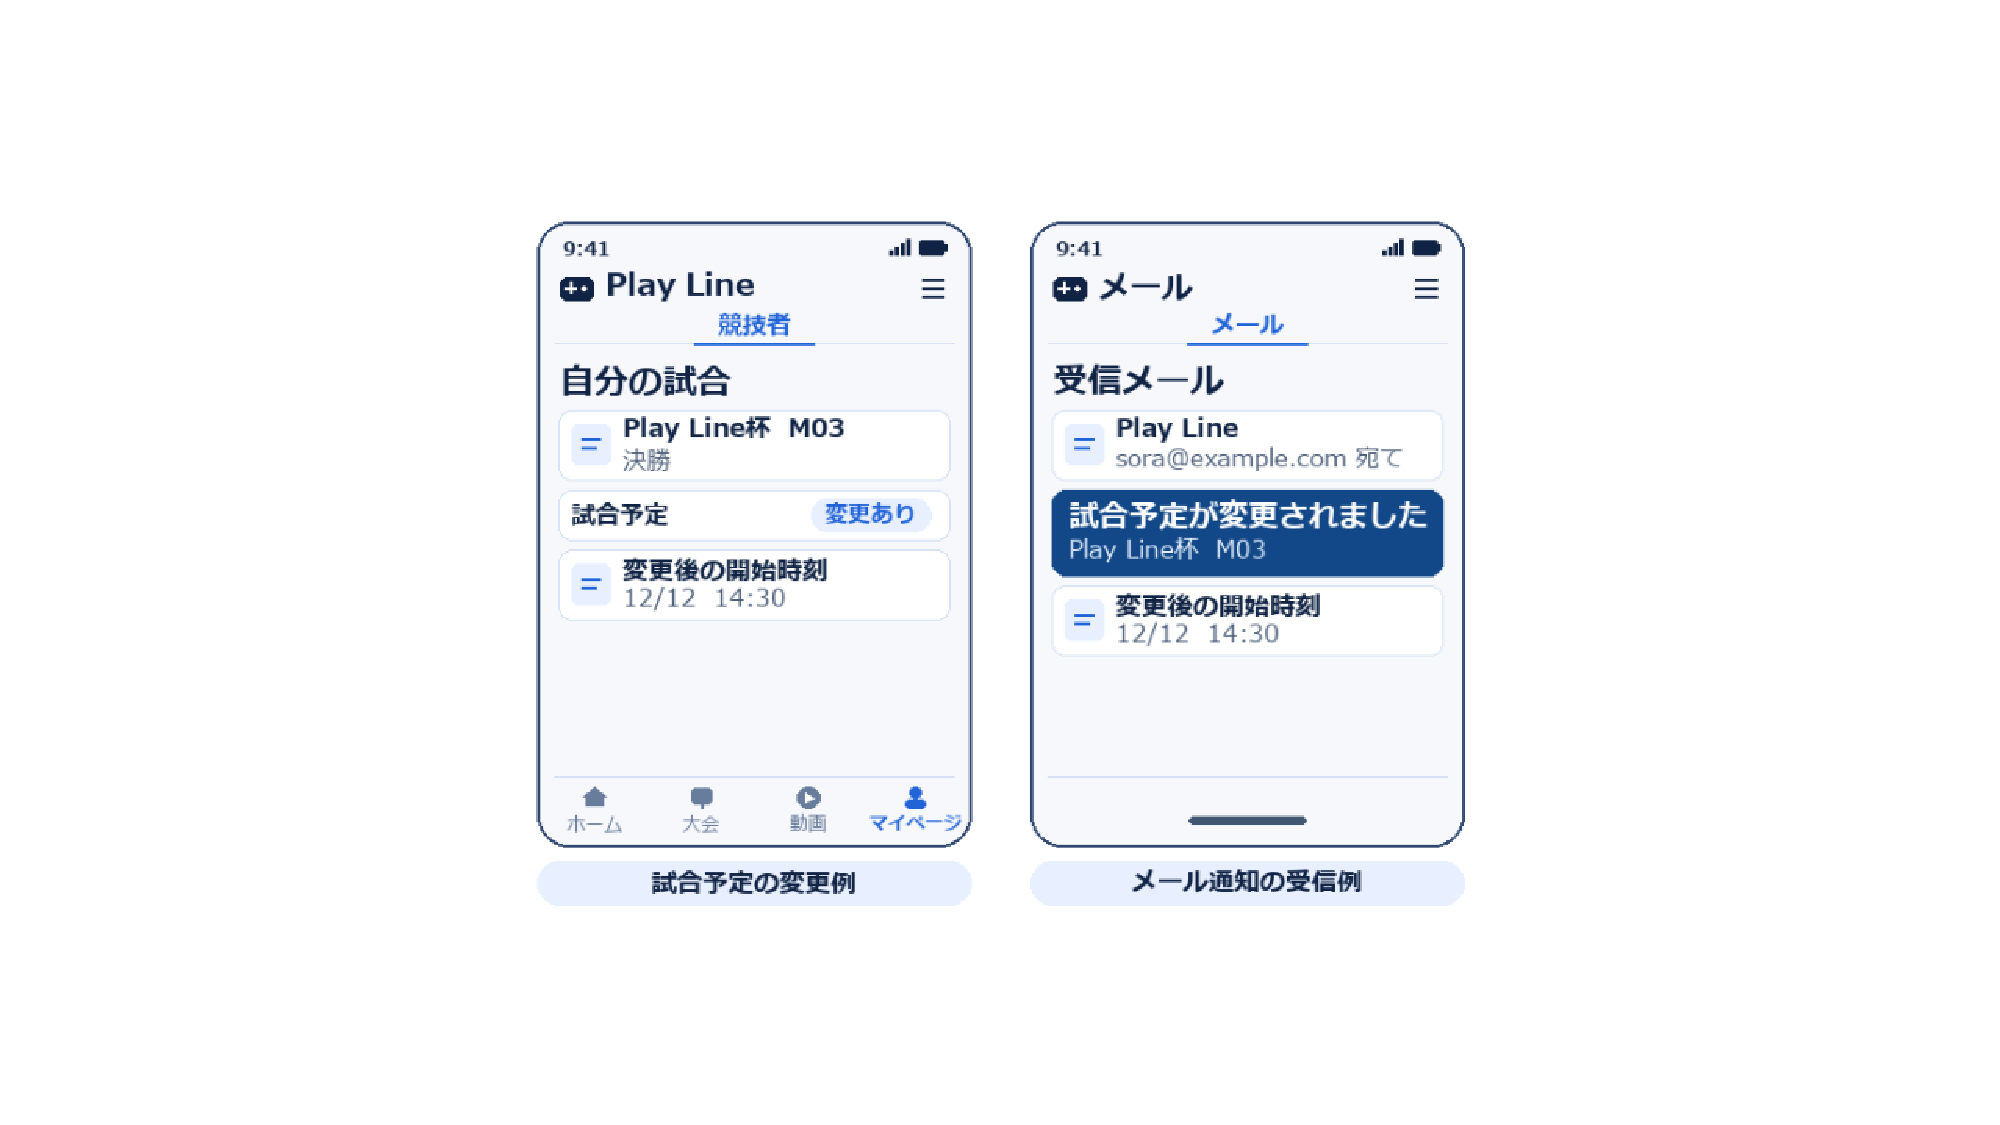
\includegraphics[width=\linewidth]{figures/03/3-5_mail.pdf}
    \caption{メール通知イメージ}
    \label{fig:notice_mail_ui}
\end{figure}

\subsubsection*{(b) お気に入り選手の配信通知機能}
\begin{description}
    \item[入力：]利用者ID、選手ID、配信情報
    \item[出力：]配信開始通知
    \item[処理：]お気に入り登録された選手の試合で配信が開始された場合、
                対象利用者にメールで通知する。
\end{description}

\begin{figure}[H]
    \centering
    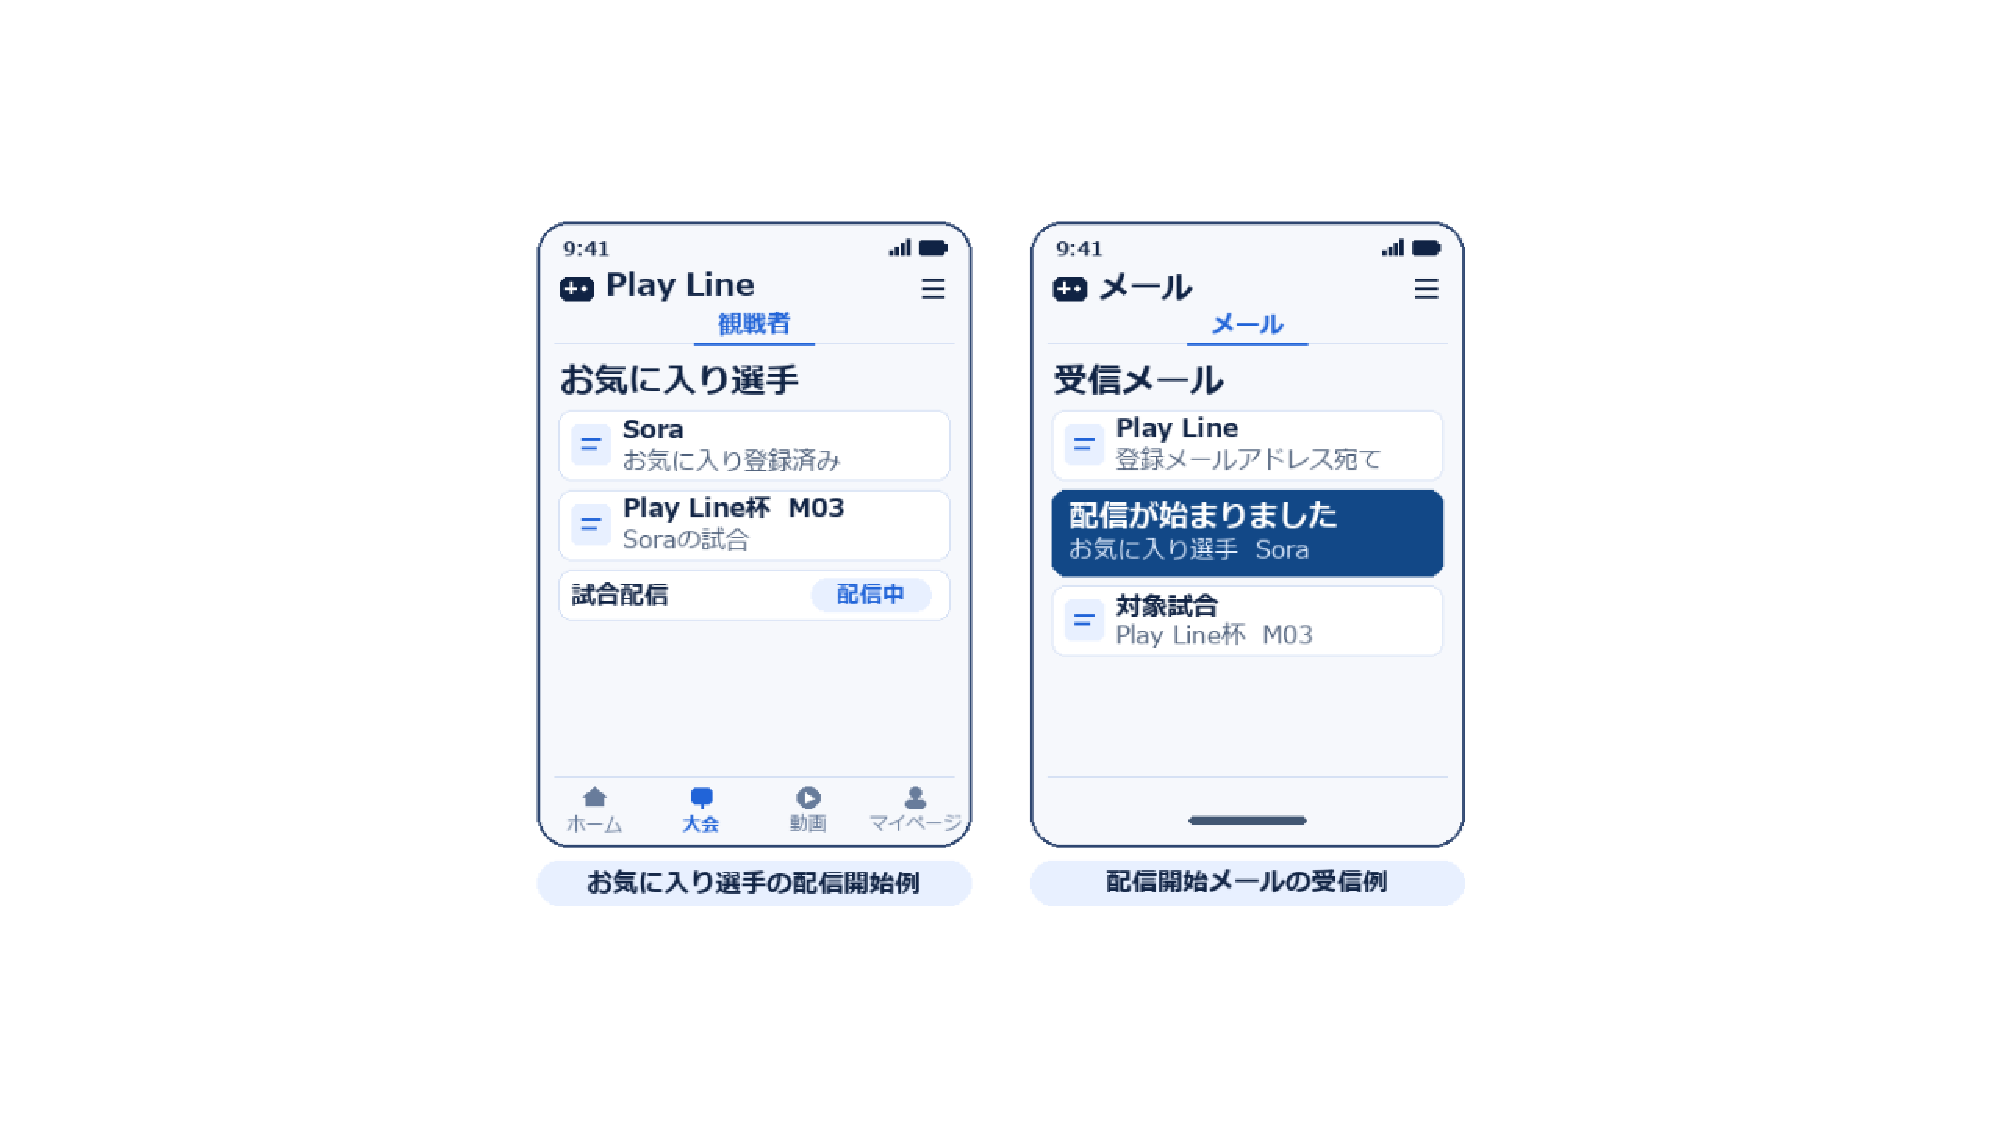
\includegraphics[width=\linewidth]{figures/03/3-5_fav_stream.pdf}
    \caption{お気に入り選手配信通知イメージ}
    \label{fig:notice_fav_stream_ui}
\end{figure}